\documentclass[
	english,
	% twoside, % print double-sided
	ruledheaders=section, % upper level where headlines are separated with lines (DEMO-TUDaPub)
	class=report,% Based document class
	thesis={type=Project Seminar Report},% document type Thesis
	accentcolor=TUDa-1d, % color scheme
	custommargins=false,% Margins are calculated automatically using typearea 
	marginpar=false,% Header and footer do not extend over the side note column
	%BCOR=5mm,%Binding correction, if necessary
	parskip=half-,%paragraph identification by spacing --> KOMA-Sript
	fontsize=11pt,%Basic font size, the corporate design font size (9pt) is often too small
%	logofile=example-image, %If the logo files are not available
]{tudapub}

% The following block is only necessary for pdfTeX on versions prior to April 2018
\usepackage{iftex}
\ifPDFTeX
	\usepackage[utf8]{inputenc}%compatibility with TeX versions before April 2018
\fi

%%%%%%%%%%%%%%%%%%%
% package suggestions mathematics
%%%%%%%%%%%%%%%%%%%
\usepackage{mathtools} % extended amsmath
\usepackage{amssymb}   % extended character set
\usepackage{siunitx}   % units
%\usepackage[bottom]{footmisc}

%%%%%%%%%%%%%%%%%%%
% Language customization & improved hyphenation rules
%%%%%%%%%%%%%%%%%%%
\usepackage[english, main=english]{babel}
\usepackage[autostyle]{csquotes}% Quotation marks simplified
\usepackage{microtype}
\usepackage{array} 
\usepackage{multirow}
\usepackage{makecell}
\usepackage{cleveref}
\crefname{lstlisting}{listing}{listings}
\Crefname{lstlisting}{Listing}{Listings}
\usepackage{wrapfig}
\usepackage{float}
\usepackage[symbol]{footmisc}
\usepackage{listings}
\usepackage{color}
\usepackage{subfig}

\definecolor{dkgreen}{rgb}{0,0.6,0}
\definecolor{gray}{rgb}{0.5,0.5,0.5}
\definecolor{mauve}{rgb}{0.58,0,0.82}

% Load the package with the acronym option
\usepackage[acronym,nomain]{glossaries}
 
\loadglsentries{acronyms}
% Generate the glossary
\makeglossaries


%%%%%%%%%%%%%%%%%%%
% bibliography
%%%%%%%%%%%%%%%%%%%
 \usepackage[backend=biber,bibstyle=ieee,citestyle=numeric-comp,url=false]{biblatex}
 \bibliography{bibliographie.bib}
\DeclareSourcemap{
  \maps[datatype=bibtex, overwrite=true]{
    \map{
      \step[typesource=misc, typetarget=online]
    }
  }
}
\DeclareDelimFormat[online]{editortypedelim}{\addspace}
\DeclareFieldFormat[online]{editortype}{}

%%%%%%%%%%%%%%%%%%%
% package suggestions tables
%%%%%%%%%%%%%%%%%%%
%\usepackage{array}     % basic package for table configuration, is loaded automatically from the following
\usepackage{tabularx}   % tables that automatically adapt to the width
%\usepackage{longtable} % Multi-Page Tables
%\usepackage{xltabular} % Multi-page tables with adjustable width
\usepackage{booktabs}   % Improved opportunities for table layout on horizontal lines

\usepackage{graphicx}
\usepackage{tikz}
%%%%%%%%%%%%%%%%%%%%%%%%%%%%%%%%%%%%%%%%%%%%%%%%%%%%%%%%%%%%%%%%%%%%%%
% LaTeX Overlay Generator - Annotated Figures v0.0.1
% Created with http://ff.cx/latex-overlay-generator/
% If this generator saves you time, consider donating 5,- EUR! :-)
%%%%%%%%%%%%%%%%%%%%%%%%%%%%%%%%%%%%%%%%%%%%%%%%%%%%%%%%%%%%%%%%%%%%%%
%\annotatedFigureBoxCustom{bottom-left}{top-right}{label}{label-position}{box-color}{label-color}{border-color}{text-color}
\newcommand*\annotatedFigureBoxCustom[8]{\draw[#5,ultra thick,rounded corners] (#1) rectangle (#2);\node at (#4) [fill=#6,thick,shape=circle,draw=#7,inner sep=2pt,font=\sffamily,text=#8] {\textbf{#3}};}
%\annotatedFigureBox{bottom-left}{top-right}{label}{label-position}
\newcommand*\annotatedFigureBox[4]{\annotatedFigureBoxCustom{#1}{#2}{#3}{#4}{white}{white}{black}{black}}
\newcommand*\annotatedFigureText[4]{\node[draw=none, anchor=south west, text=#2, inner sep=0, text width=#3\linewidth,font=\sffamily] at (#1){#4};}
\newenvironment {annotatedFigure}[1]{\centering\begin{tikzpicture}
\node[anchor=south west,inner sep=0] (image) at (0,0) { #1};\begin{scope}[x={(image.south east)},y={(image.north west)}]}{\end{scope}\end{tikzpicture}}
%%%%%%%%%%%%%%%%%%%%%%%%%%%%%%%%%%%%%%%%%%%%%%%%%%%%%%%%%%%%%%%%%%%%%%



\usepackage{pifont}% Zapf-Dingbats symbols
\newcommand*{\FeatureTrue}{\ding{52}}
\newcommand*{\FeatureFalse}{\ding{56}}

\newcommand{\textoverline}[1]{$\overline{\mbox{#1}}$}
\newcommand{\inlcode}[1]{\textit{\detokenize{#1}}}
\newcommand{\taglg}[1]{\textless {#1}\textgreater}

\lstset{frame=tb,
  xleftmargin=2em,
  framexleftmargin=2em,
  language=Verilog,
  captionpos=b,
  aboveskip=3mm,
  belowskip=3mm,
  showstringspaces=false,
  columns=flexible,
  basicstyle={\small\ttfamily},
  numbers=left,
  rulecolor=\color{gray},
  numberstyle=\tiny\color{gray},
  keywordstyle=\color{blue},
  commentstyle=\color{dkgreen},
  stringstyle=\color{mauve},
  breaklines=true,
  breakatwhitespace=true,
  escapechar=~,
  tabsize=3
}
\makeatletter
\let\orig@lstnumber=\thelstnumber

\newcommand\lstsetnumber[1]{\gdef\thelstnumber{#1}}
\newcommand\lstresetnumber{\global\let\thelstnumber=\orig@lstnumber}
\makeatother
%\usepackage{caption}
%\captionsetup{justification=raggedright,singlelinecheck=false, margin=2em, format=plain}
%\captionsetup[lstlisting]{margin=2em}

\RedeclareSectionCommand[
  runin=false,
  beforeskip=-.5\baselineskip,
  afterskip=-.1\baselineskip
]{subsubsection}

\begin{document}

\Metadata{
	title = Design and Development of a Custom ASIC Test PCB for Ultrasonic Communication,
	author = Malte Nilges
}

%%%%%%%%%%%%%%%%%%%
%Fill in the missing Information
%%%%%%%%%%%%%%%%%%%
\title{Design and Development of a Custom ASIC Test PCB for Ultrasonic Communication}
% \subtitle{}
\author{\\ Malte Nilges, 2704362}
% \birthplace{birthplace}
% \reviewer{Reviewer 1 \and Reviewer 2 ...}%Reviewer

\department{etit}  % Will be automatically replaced 
% \institute{institute}
% \group{group}

\institute{\hspace{0.1cm}\\\centering
\includegraphics[width=2.5cm]{logo/ies_logo}} % smal Hack for the logo

\submissiondate{\today}
% \examdate{\today}

\subtitle{
Course Semester: SS 2023\\
Supervisor: Dominic Korner\\
Department: Integrierte Elektronische Systeme (IES)\hfill\textbar\hfill Prof.\,Dr.-Ing.\, Klaus Hofmann}


\maketitle


% \affidavit  % till now only available in German

% Table of contents:
\tableofcontents


% Chapters:
% -------------------------------------------------------------------
\chapter{Introduction}

The work presented in this report is part of a project seminar conducted in the \gls{IES} lab at the Technical University of Darmstadt. This chapter gives an overview of the purpose and objectives of the project seminar and some physical background knowledge relating to the project.

\section{Overview}\label{sec:overview}
Systems that perceive and evaluate their targeted environment rely on the usage of sensors to acquire the desired data. For many sensing applications, including the monitoring of structures, machinery, the environment, or human health, wireless sensor communication is an essential part of such systems as it is often the only feasible way to share acquired data to other systems or human operators  \autocite{dargieFundamentalsWirelessSensor2010}.

There are different methods of wireless sensor communication, which differ in frequency, range, data rate and energy consumption. Some examples for commonly used technologies are Bluetooth, ZigBee, WLAN or ultrasonic communication. Common to all is that energy is required in order to communicate. In scenarios where the usage of batteries is not possible, that energy needs to be harvested from the surroundings, e.g. from electrical signals transmitted to the system or from mechanical forces exerted on the system. This method is called energy harvesting or \gls{WPH}. Depending on the environment, different communication and \gls{WPH} techniques are suited. Criteria may be the environment, the available space, the density of the transmission medium and the transmission range \autocite{valentaHarvestingWirelessPower2014}.

The objective of this work is to enable communication and energy transmission using ultrasound, which means sound waves with frequencies greater than the audible frequency range of about \SI{20}{\kilo\hertz}. These mechanical vibrations are transported through a transmission medium such as air or metal.
Piezoelectric transducers are capable to both transmit and receive ultrasound waves and therefore the method of choice for the targeted functionality. Such components are constructed of materials that change in shape when an electric field is applied (piezoelectric actuator) and generate an electric fields when exposed to a deforming mechanical force (piezoelectric sensor). As this process is reversible, piezoelectric materials can act both as sensors and actuators \autocite{vivesPiezoelectricTransducersApplications2008}.

In order to perform a two-way communication, the system designed in this work must be able to connect the piezo element to a \gls{VCVS} in order to apply an electric field resulting in ultrasonic vibrations, as well as receive, amplify and process the electric signals that are induced by the piezo element when exposed to ultrasonic vibrations. The input signal processing needs to 1) convert the amplified signal into a digital code in order to detect its amplitude and 2) determine the frequency with a sufficient accuracy in order to detect changes for frequency modulated signals. The intended solution for this task is the usage of an \gls{ADC} and a comparator. A further requirement is a system for communicating with an external machine in order to receive commands and transmit sampled data.

The implementation of this abstract system is described in \cref{chap:impl}.

\section{Piezoelectric effect}
The phenomenon of an electric field being generated in a material when it is subjected to mechanical stress or strain is known as the piezoelectric effect. Its counterpart is the inverse piezoelectric effect due to which a mechanical strain or deformation occurs in a material when it is subjected to an electric field \autocite{wangPiezoelectricPiezotronicEffects2013,arnauFundamentalsPiezoelectricity2008}.

The piezoelectric effect is only exhibited by crystalline materials which either lack a center of symmetry in their atomic structure or exhibit a dipole moment that can be polarized (so-called ferroelectrics). Crystals are materials that have a uniform atomic structure called lattice which extends in all directions of the material. On a macroscopic level, the lattice of a single crystal is visible by the orientation of its flat faces. The counterpart to crystalline structures are amorphous structures, which have no periodicity in their atomic arrangement.
In semiconductor technology, the crystalline structures of materials such as silicon are deliberately disrupted by adding impurities, called dopants, in order to create semiconductors such as diodes.

Piezoelectric materials rely on non-centrosymmetric crystalline structures, meaning that the ions are distributed without a center of symmetry. In such materials, the polarization changes as a force such as compression, expansion, tension or torsion, depending on the crystal lattice, is applied. The force has to be directed for a change in polarization, as the lattice is not asymmetrical in every dimension. Inside the material, facing ions may cancel may cancel each other, but the change of the polarization appears as a positive and negative charge on the surfaces generating an electrostatic output voltage. Due to internal leakage paths formed by impurities, the voltage drops after some time\autocite{arnauFundamentalsPiezoelectricity2008,grinerPiezoelectricMaterials2016}.

Typical examples for piezoelectric materials include monocrystalline materials like Rochelle salt or quartz, but also polycrystalline ferroelectric ceramics such as lead zirkonate titanate (PZT). Materials of latter category need to be polarized first. This process is performed using a high electric field at temperatures close to the Curie-temperature at which the ferroelectric properties of the material would disappear. The otherwise randomly orientated dipoles align with the electric field forming a permanent dipole and the material becomes piezoelectric \autocite{kimPiezoelectricEnergyHarvesting2009,grinerPiezoelectricMaterials2016}.

\Cref{drw:piezo_effect} shows the piezoelectric effect on a molecular model. As a force is applied to the molecule, the positive and negative gravity centers of the molecules are seperated, generating a dipole and thus an electric field.
\begin{figure}[H]
    \centering
    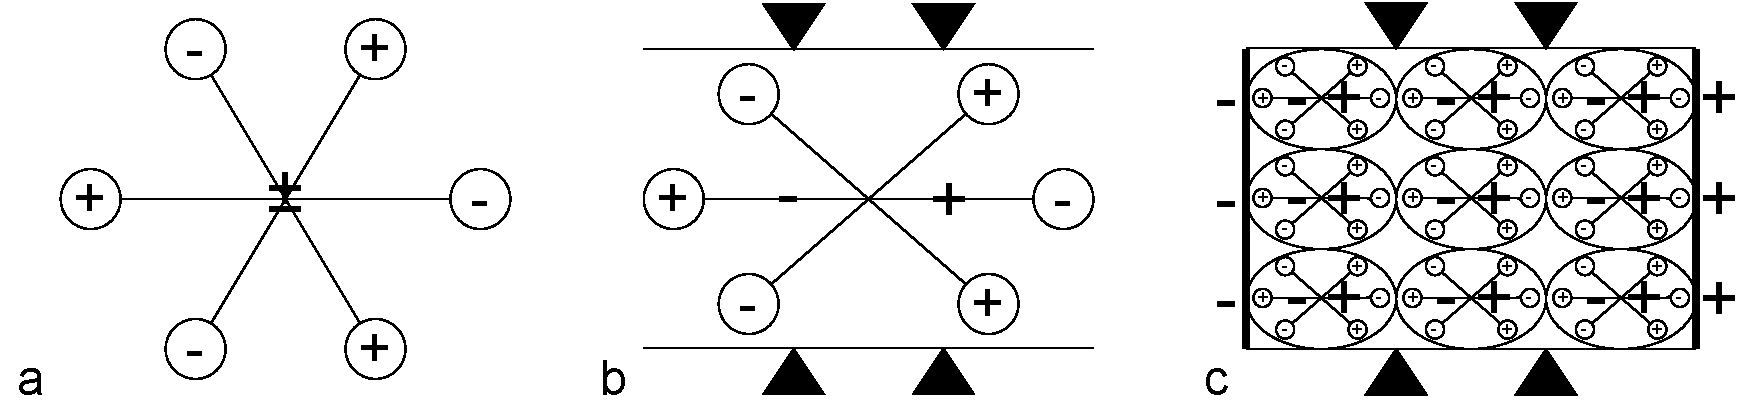
\includegraphics[width=\columnwidth]{drawings/piezoelectric_effect.pdf}
    \caption{Model of the piezoelectric effect: a) unperturbed molecule; b) molecule exposed to force; \\c) surface of a material exposed to force}
    \label{drw:piezo_effect}
\end{figure}

Piezo elements have one or multiple resonance frequencies, at which their induced electric signal resulting from a mechanical force is highest and vice versa. The resonance effect is caused by the ability to transfer energy between the storage modes of electric and vibrational energy as described above. At resonance, the damping is lowest, hence the exerted energy is stored and rising with each oscillation. As realistic systems have always some kind of damping e.g. in form of friction, the maximum stored energy is limited, but yet it can be high enough to destroy the material e.g. due to tension caused by movements or due to breakdown voltages. The damping can be described by the quality factor Q, which is defined  as the resonance frequency divided by the resonance width, being the bandwidth, over which the power is more than half compared to that of resonance. A high Q means less damping but also a lower relative resonance width, making the system more selective. For optimal energy transmission, the piezo element should be driven near its resonance frequency \autocite{arnauFundamentalsPiezoelectricity2008,lucklumModelsResonantSensors2008}.

\chapter{Implementation}\label{chap:impl}

\begin{wrapfigure}{L}{.6\columnwidth}
    \vspace{-13pt}
    \centering
    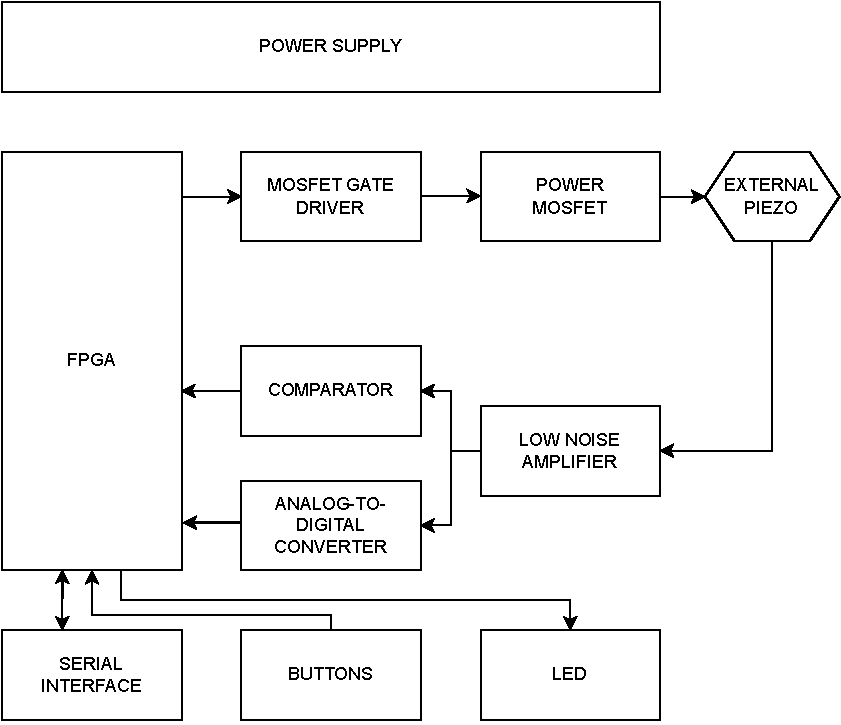
\includegraphics[width=.55\columnwidth]{drawings/overview.pdf}
    \caption{System overview as data flow diagram}
    \label{drw:overview}
    \vspace{-40pt}
\end{wrapfigure}

The test platform for ultrasonic communication was implemented according to the objectives specified in \cref{sec:overview}. The implementation consists of two parts, the hardware platform, executed as a custom \gls{PCB} design, and the software platform, containing the logic to control the circuit and to send, receive and process data. \Cref{drw:overview} shows a data flow diagram of the resulting system, the controlling of each system part is performed by the \gls{FPGA}.

The following sections describe the designed hardware and software. Please refer to \cref{chap:results} for the results and a discussion of the proposed system.
\\\\\\


\section{Hardware platform}
Since a platform for controlling a piezo element was already available, it was used as the basis for all modifications and extensions. The existing hardware platform consisted of a driver stage to use the piezo element as an actuator, an amplifier stage in case of data reception and a connector for a Digilent CMOD S7 \gls{FPGA} development board to control the driver stage and to adjust the amplifier stage.

This basic structure was retained, but the driver stage was replaced to meet the changed output power requirements and an \gls{ADC} and comparator stage was added to process and forward received data in digital form. The \gls{PCB} design was performed with the use of the circuit design tool KiCAD 6.0.

\subsection{Piezo driver stage}\label{sec:driverschem}
The driver stage is responsible for properly exciting the piezo transducer and was designed with the following specifications in mind:
\begin{itemize}
  \item \SI{1}{\mega\hertz} to \SI{2}{\mega\hertz} switching frequency
  \item \SI{38}{\volt} input voltage to the piezo transducer
  \item \SI{100}{\ohm} equivalent load
\end{itemize}

The original driver stage was based on a Microchip TC6320, a complementary N- and P-channel \gls{MOSFET} pair supporting voltages of \SI{\pm100}{\volt} and currents of at least \SI{2}{\ampere} \autocite{microchiptechnologyinc.NChannelPChannelEnhancementMode2017}. Despite being classified as a power transistor pair, the circuit has the disadvantage of a rather high R\textsubscript{DS,ON} resistance, which, depending on the applied gate-to-source voltage, is at least \SI{7}{\ohm} in the case of the NMOS and at least \SI{8}{\ohm} in case of the PMOS and must therefore be cooled accordingly for larger currents. 
In order to circumvent the thermal limitation of the existing driver stage, it was revised and improved. Two separate onsemi FDD1600N10ALZ N-channel \glspl{MOSFET} \autocite{onsemiconductorcorporationNChannelPowerTrenchMOSFET2014} with an R\textsubscript{DS,ON} resistance of \SI{150}{\milli\ohm} and similar input capacitance C\textsubscript{iss} of \SI{169}{\pico\farad} are providing lower conduction losses while maintaining the same switching loss.

\begin{figure}[H]
    \centering
    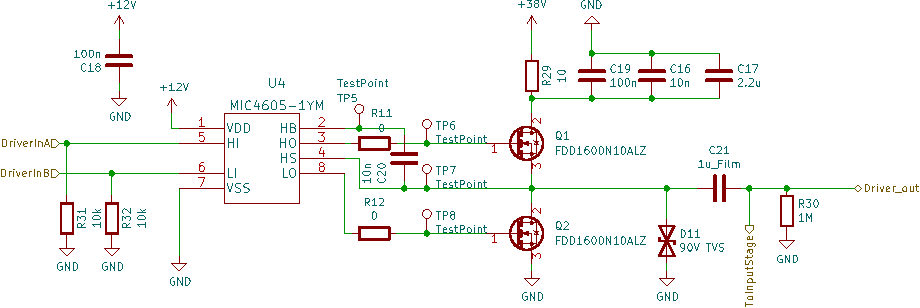
\includegraphics[width=0.8\columnwidth]{schematics/sch_driver.pdf}
    \caption{Piezo driver stage}
    \label{sch:driverstage}
\end{figure}

The gate driver is a Microchip MIC4604 featuring two outputs and an integrated bootstrap diode for driving N-channel \glspl{MOSFET} in half-bridge configuration \autocite{microchiptechnologyinc.85VHalfBridgeMOSFET2018}. An external bootstrap capacitor is used to boost the voltage at the high-side gate of the \gls{MOSFET}. The gate driver is controlled by two separate inputs, the timing to avoid shoot-through, meaning a short circuit from V\textsubscript{in} to ground due to simultaneously active \glspl{MOSFET}, is performed by software. In case of data reception, both half-bridge \glspl{MOSFET} can be switched off in order to avoid a load on the signal source and cross-talk in the received signal.

The output of the signal to the piezo is filtered by a RC high-pass. The coupling capacitor was designed with \SI{1}{\micro\farad}, the resistor with \SI{100}{\mega\ohm}.

\subsection{Input stage and amplifier}

\begin{figure}[H]
    \centering
    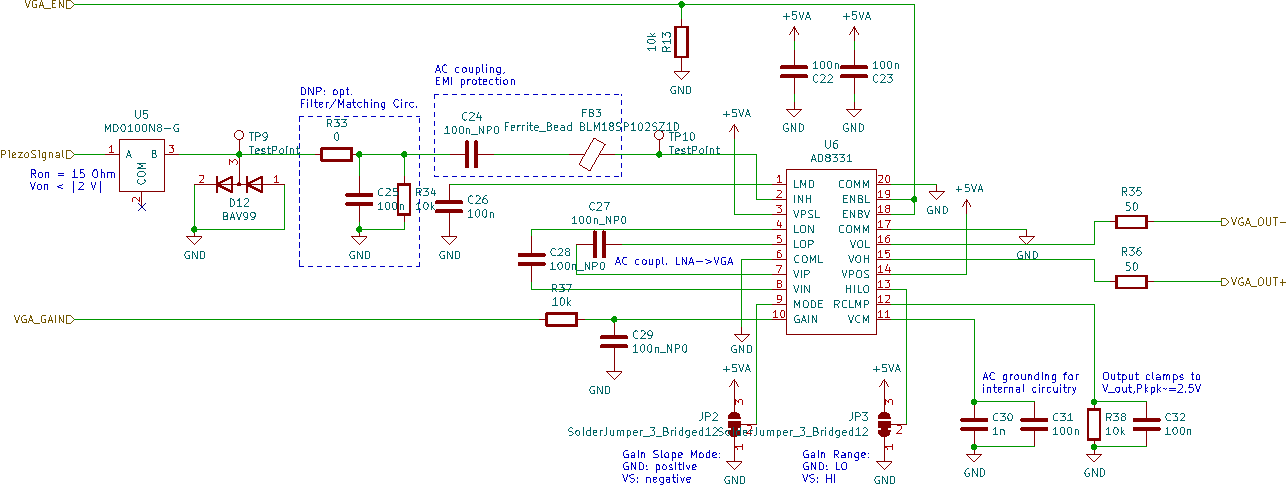
\includegraphics[width=1.0\columnwidth]{schematics/sch_inputstage.pdf}
    \caption{Input stage and amplifier schematic}
    \label{sch:inputstage}
\end{figure}
The input stage was largely taken over from the original version. Since the same piezo transducer is used for transmitting and receiving and thus the transmit path is electrically connected to the receive path, a Microchip MD0100 T/R switch was used which has been explicitly designed for ultrasonic applications \autocite{microchiptechnologyinc.SingleDualChannelHighVoltage2018}. The switch protects the \gls{LNA} from high input voltages that would occur in the event of a transmit signal. Once the voltage between input and output exceeds \SI{\pm2}{\volt}, the switch turns off, limiting the current to \SI{200}{\micro\ampere}. The switching time is \SI{20}{\nano\second}, for faster transients and to limit the \gls{LNA} input, anti-parallel Schottky diodes with short reverse recovery times t\textsubscript{rr} are used in the form of the Vishay BAV99 integrated circuit \autocite{vishaysemiconductorSmallSignalSwitching2018}.

In series to the \gls{LNA} input is an additional passive filter network which can be modified to adjust the frequency components to be amplified, although it is not placed in order to avoid additional noise from being amplified. A coupling capacitor and a ferrite provide for the filtering of DC components and high-frequency interference signals, respectively.

The amplifier itself is an Analog Devices AD8331 \autocite{analogdevicesUltralowNoiseVGAs2016}. This circuit connects a \gls{LNA}, which has a fixed gain of \SI{19}{\decibel}, to a \gls{VGA} with an adjustable gain between \SI{-4.5}{\decibel} and \SI{43.5}{\decibel} in LO gain mode and between \SI{7.5}{\decibel} and \SI{55.5}{\decibel} in HI gain mode. The \SI{3}{\decibel} bandwidth is \SI{120}{\mega\hertz} and is thus well suited for amplification of high frequency signals. The gain is set by the gain pin and a 4-bit \gls{DAC}, implemented as a resistor network, provides the intended voltage level between \SI{0}{\volt} and \SI{1}{\volt}. The differential peak-to-peak output is limited to \SI{2.5}{\volt} by the Rclmp pin to protect downstream components and is terminated with \SI{50}{\ohm} resistors.

The amplified signal can then either be output via the BNC connectors or, alternatively, processed further in digital form using the analog-to-digital converter or the comparator.

\subsection{Analog-to-digital converter}

\begin{figure}[H]
    \centering
    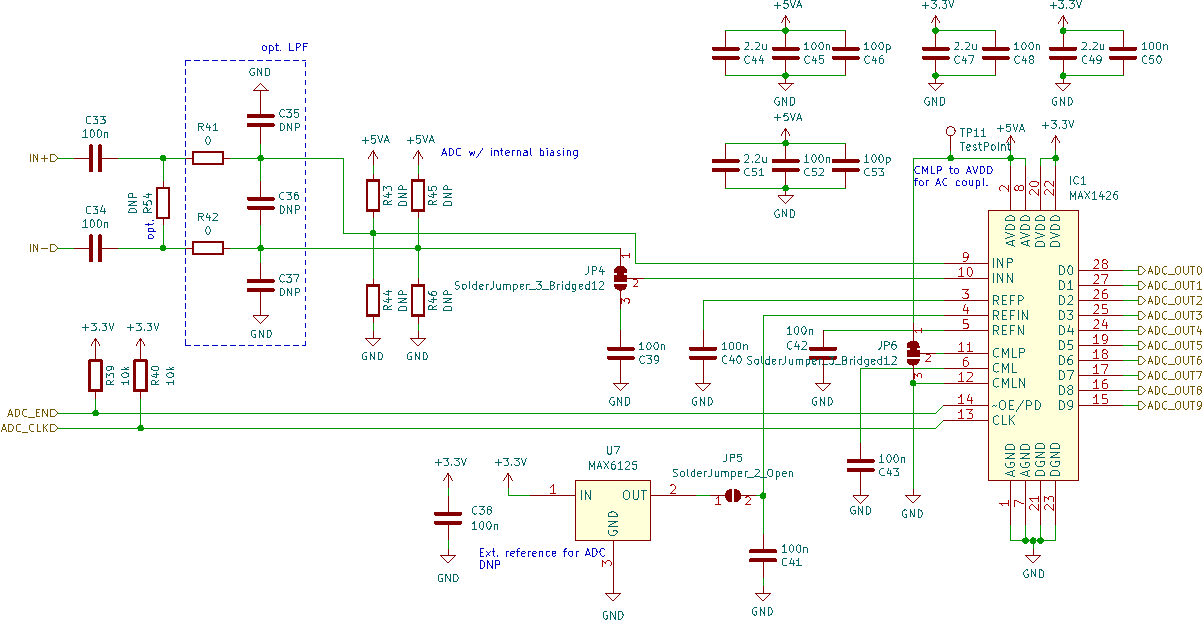
\includegraphics[width=1.0\columnwidth]{schematics/sch_adc.pdf}
    \caption{\gls{ADC} schematic}
    \label{sch:adc}
\end{figure}
Analog Devices' MAX1426 analog-to-digital converter is a 10 bit, 10 megasamples per second pipeline \gls{ADC} \autocite{analogdevices10Bit10MspsADC2011}. It supports a differential signal that is superimposed in the case of AC coupling using an integrated common-mode voltage. This bias voltage is \SI{2.25}{\volt} at the CML pin, which is derived from an internal or external voltage reference of \SI{2.5}{\volt}. The reference voltages required for comparison are \SI{3.25}{\volt} (REFP pin) and \SI{1.25}{\volt} (REFN pin). Thus, the input range is \SI{\pm2}{\volt}. Alternatively, the bias voltage and reference voltages can be specified by applying appropriate voltage levels to the pins themselves, although this is not implemented in the board design.

The digital output signal is provided via a parallel interface in two's complement. Because of the separate supply voltages for the analog and digital sections, the output level is set to \SI{3.3}{\volt}, eliminating the need to convert the logic level externally. The latency between input and output signal is 5.5 clock cycles.

\subsection{Comparator}

\begin{figure}[H]
    \centering
    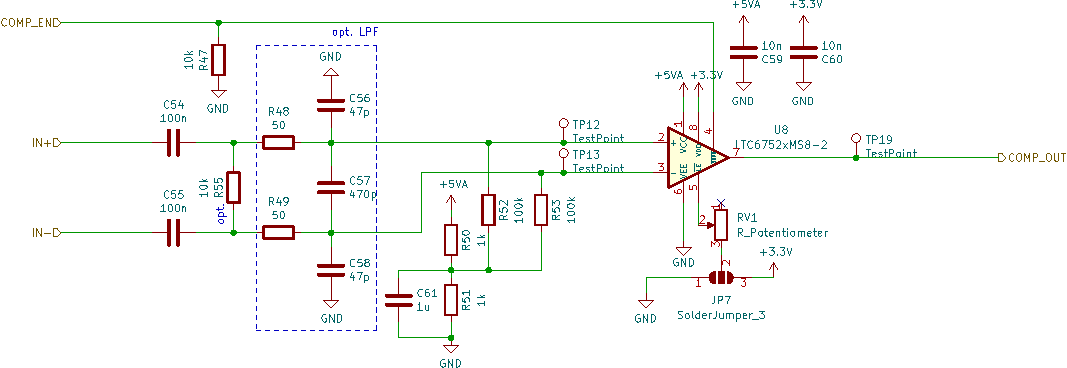
\includegraphics[width=1.0\columnwidth]{schematics/sch_comparator.pdf}
    \caption{Comparator schematic}
    \label{sch:comparator}
\end{figure}
The comparator is an Analog Devices LTC6752 featuring toggle rates of up to \SI{280}{\mega\hertz} and low propagation delay as well as low rise and fall times in the range of a few nanoseconds \autocite{analogdevices280MHz9nsComparator2014}. It is supposed to enable the possibility of transmitting data with frequency modulation by counting the number of the respective \gls{FPGA} clock cycles in order to determine the transmission of a '0' or a '1'. The device features differential inputs and separate supply rails for the input and output stage. After the AC-coupling of the signal coming from the \gls{VGA}, the differential signal is filtered with a passive band-pass filter which suppresses noise from unwanted frequencies. The \SI{3}{\decibel} corner frequencies are calculated as follows:
\[f_{3dB,CM}^{HPF} = \frac{1}{2\pi C_{in} R_{CM}}\approx \frac{1}{2\pi \cdot \SI{100}{\nano\farad} \cdot \SI{100}{\kilo\ohm}} = \SI{15.92}{\hertz}\]
\[f_{3dB,CM}^{LPF} = \frac{1}{2\pi R_{in} C_{CM}}\approx \frac{1}{2\pi \cdot \SI{50}{\ohm} \cdot \SI{47}{\pico\farad}} = \SI{67.73}{\mega\hertz}\]

\[f_{3dB,DM}^{HPF} = \frac{1}{2\pi \cdot C_{in} \left( \frac{1}{2}R_{DM} \| R_{CM} \right)}\approx \frac{1}{2\pi \cdot \SI{100}{\nano\farad} \cdot \left( \SI{5}{\kilo\ohm} \| \SI{100}{\kilo\ohm} \right)} = \SI{334.23}{\hertz}\]
\[f_{3dB,DM}^{LPF} = \frac{1}{2\pi \cdot R_{in} \left( 2C_{DM}+C_{CM} \right)}\approx \frac{1}{2\pi \cdot \SI{50}{\ohm} \cdot \left( \SI{940}{\pico\farad} + \SI{47}{\pico\farad} \right)} = \SI{3.23}{\mega\hertz}\]

%passive BPF advantages: easy filtering, downsides: less gain -> less SNR, bad selectivity (low Q), perfect filters rely on 0 ohm output freq and no loading, with cascaded filters this is not the case and the filters influence each other
%https://electronics.stackexchange.com/questions/185172/passive-filter-design-transfer-functions-and-loading

After filtering, the AC signal is biased to a DC operating point of \SI{2.5}{\volt}, generated by a voltage divider of the \SI{5}{\volt} analog supply rail \autocite{analogdevicesBiasingDecouplingOp}.
%https://e2e.ti.com/support/power-management-group/power-management/f/power-management-forum/670293/voltage-reference-for-comparator-input-biasing-low-output-resistance

In order to further minimize the effect of noise at the cost of latency, the comparator provides an adjustable hysteresis, meaning different tripping points for a positive and negative input voltage difference in order to change the output. The internal hysteresis is set by using an external resistor between the input of the \textoverline{LE}/HYST-Pin and GND. The default value is \SI{5}{\milli\volt} and increases as the voltage of the pin is being decreased from its default open loop value of \SI{1.25}{\volt}. By pulling the \textoverline{LE}/HYST-Pin to VCC the hysteresis could also be eliminated. As we are dealing with amplified and comparatively slow signals, the hysteresis is set to around \SI{20}{\milli\volt} using a potentiometer in order to get a steady signal at the output when there is no substantial difference voltage at the input, i.e. in the case of no signal.

\subsection{FPGA and I/O}

\begin{figure}[H]
    \centering
    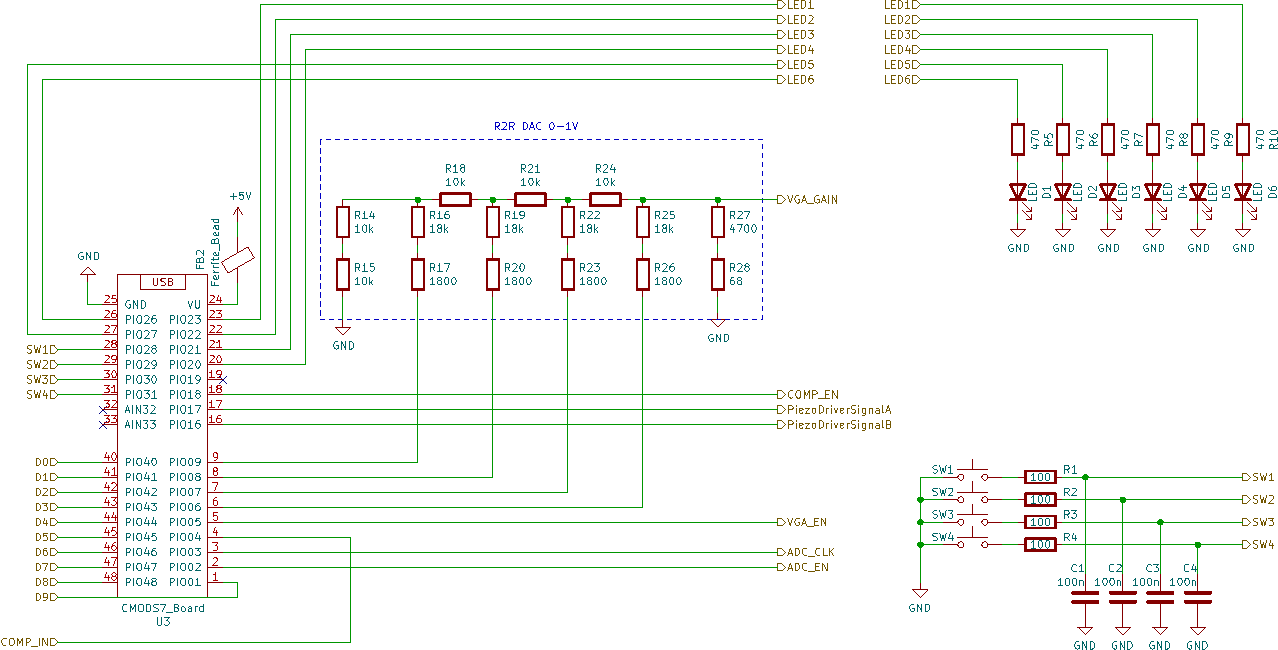
\includegraphics[width=1.0\columnwidth]{schematics/sch_fpga.pdf}
    \caption{\gls{FPGA} and I/O schematic}
    \label{sch:fpga}
\end{figure}
In order to reduce the individual component count on the \gls{PCB} and to enable easier replacements, a breadboardable \gls{FPGA} module in form of the CMOD S7 was chosen to provide the logic functionality for the communication platform \autocite{digilentBreadboardableSpartan7FPGA}. It features a Xilinx Spartan7 XC7S25 \gls{FPGA} on a 48-pin \gls{DIP} form factor board driven by a \SI{12}{\mega\hertz} external clock and a FTDI FT2232HQ USB-UART bridge for communication with a host computer. The \gls{FPGA} module requires a \SI{5}{\volt} supply voltage, which is either provided by an USB connection or using the \SI{5}{\volt} digital supply rail, which is decoupled and filtered in order to reduce effects on the analog rail sourced from the same \gls{LDO}.

Of the 36 pins of the module, 32 are usable as digital inputs or outputs, not counting the pins of the additional PMOD header on the board. The pins are connected to the \gls{FPGA} via \SI{240}{\ohm} series resistors, limiting the switching speed to \SI{25}{\mega\hertz}, which is sufficient for driving and polling all circuits on the board. Besides the control of the platform over serial communication, some basic functionality should be accessible without the need of an external computer, hence four switches have been placed on the board in addition to the two switches included on the CMOD S7. These external buttons are pulled to VDD internally and connect the pins to GND in case of a button press. The debouncing of a button press is performed in logic, but the board provides the option to replace the arbitrarily chosen RC network in order to perform the debouncing via hardware. For basic output, six \glspl{LED} have been placed on the board, which together with the \glspl{LED} of the module sums up to a total of ten single color \glspl{LED} plus one RGB \gls{LED}.

The \gls{VGA} requires a voltage between \SI{0}{\volt} and \SI{1}{\volt} in order to control the gain of the differential output stage. This is achieved by a 4 bit R-2R-Ladder \gls{DAC} with a voltage divider at its output, giving the option to control the gain from logic if needed. The \gls{DAC} features 16 steps with a step size around \SI{66.6}{\milli\volt}, with pin PIO9 controlling the \gls{LSB} and PIO6 controlling the \gls{MSB}. The resistor values have been reused from the original design and simulated in LTSpice for verification.

Besides the \gls{IO} and the 4 bit \gls{DAC}, the \gls{FPGA} provides the enable signals of the \gls{VGA}, the \gls{ADC} and the comparator, the clock for the \gls{ADC} and the high-side and low-side signals for the piezo driver stage and receives the parallel 10 bit output signals from the \gls{ADC} and the 1 bit comparator output.

\subsection{Power supply}

\begin{figure}[H]
    \centering
    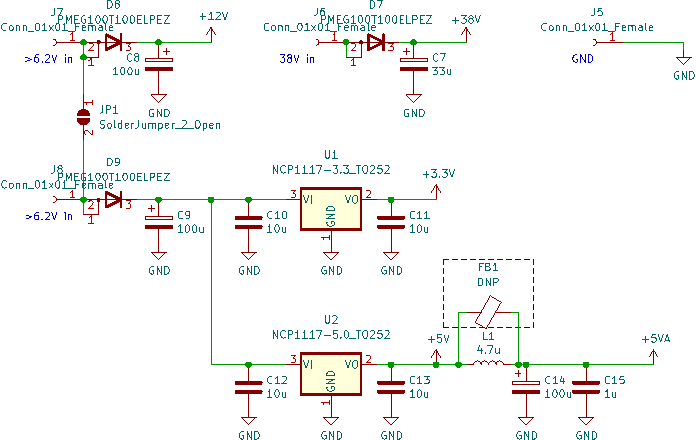
\includegraphics[width=0.8\columnwidth]{schematics/sch_power.pdf}
    \caption{Power supply schematic}
    \label{sch:power}
\end{figure}
The power stage features three different supply voltage inputs in addition to a common ground connection. All inputs are protected against reverse polarity by nexperia PMEG100 general purpose Schottky barrier rectifier with a forward voltage drop of \SI{750}{\milli\volt} \autocite{nexperia10010Low2020}. The first input supplies the two onsemi NCP1117-3.3 and NCP1117-5 \glspl{LDO}, providing stable \SI{3.3}{\volt} and \SI{5}{\volt} references respectively \autocite{onsemiconductorcorporationLowDropoutPositiveFixed2017}. In order to compensate the voltage drop of the reverse polarity protection diode and to meet the specifications of the \SI{5}{\volt} \gls{LDO}, the input voltage at the connector should be greater than \SI{6.2}{\volt}. According to the recommended application, the \glspl{LDO} are decoupled with \SI{10}{\micro\farad} ceramic capacitors. As the \SI{5}{\volt} \gls{LDO} has to supply digital logic which can lead to increased noise due to high switching frequencies, the analog rail is filtered using an LC low-pass filter in addition to the usage of a ferrite bead connected to the VU pin of the \gls{FPGA} module. The \SI{3.3}{\volt} rail is for digital signals only. The other two voltage inputs supply the gate driver, which requires a gate drive supply voltage between \SI{5.5}{\volt} and \SI{16}{\volt}, depending on the desired gate voltage and the resulting R\textsubscript{DS,ON} resistance, as well as the driving voltage for the piezo transducers, which is specified to be around \SI{38}{\volt}. The gate driver voltage input can be shorted to the \gls{LDO} voltage input, if only two DC power supplies are desired and the thermal budget of the \glspl{LDO} is not exceeded.

\subsection{PCB design}

\begin{figure}[H]
    \centering
    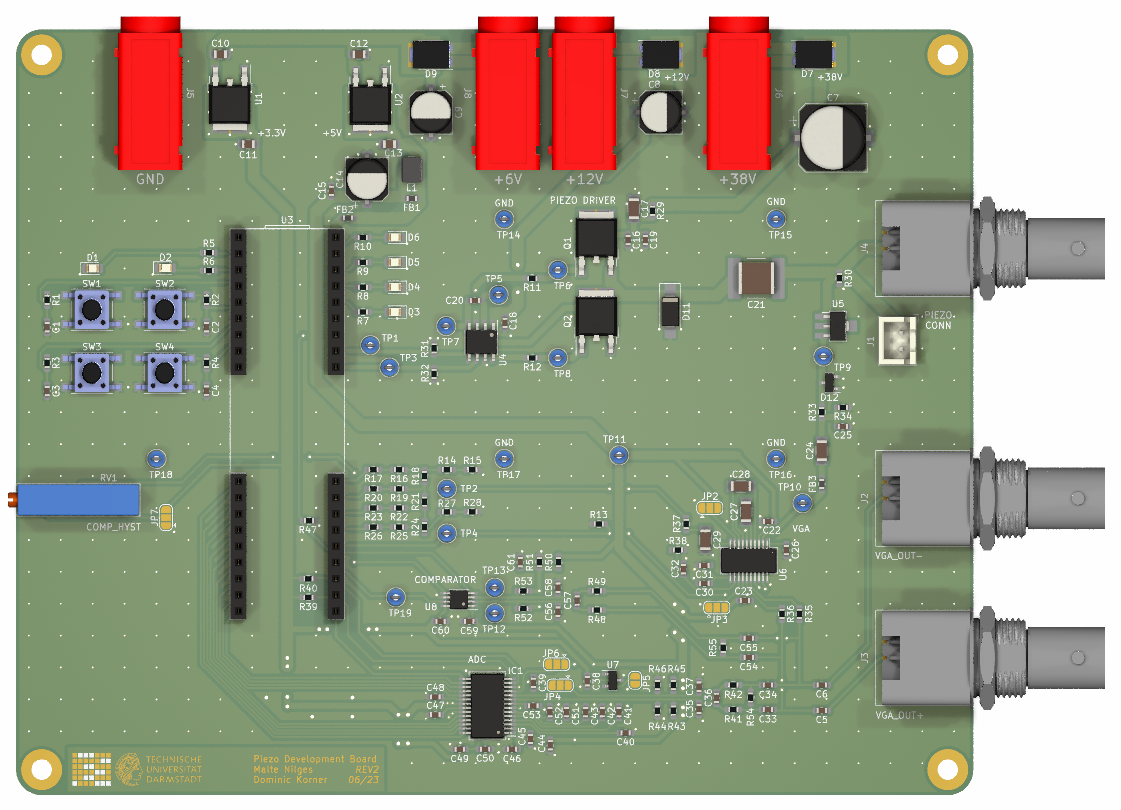
\includegraphics[width=0.8\columnwidth]{schematics/Piezo_DevBoard1.png}
    \caption{PCB Rendering}
    \label{sch:render}
\end{figure}
The \gls{PCB} layout is based on a simple two layer board with dimensions of \SI{150}{\milli\m} x \SI{120}{\milli\m}, executed in a horizontal layout. As the signals on the board are on the lower \SI{}{\mega\hertz} region and the component size and density do not require a high trace density, a two layer design approach was chosen, as it is the most efficient choice in terms of design time, production time and cost. The bottom layer acts as a ground plane with little breaks for routing in order to create a low impedance return path and to avoid large loop inductance which may lead to noise negatively effecting the AC performance of the board \autocite{mardiguianControllingRadiatedEmissions2014}. The top layer is used for component placement and signal routing with a densly stitched copper pour to the ground plane which avoids the risk of bending due to uneven copper distribution and may improve radiation of high speed digital signals.

The power section was placed on the upper section of the board, with the common ground connector on the left, and the other DC voltage connectors placed to the right alongside their respective decoupling capacitors and \glspl{LDO}. The \glspl{LDO} are stitched to small copper pours on the bottom layer to improve thermal dissipation. The 48-pin \gls{DIP}-sized CMOD S7 has only 36 pins, hence the footprint has been replaced with two 18-pin \gls{DIP} footprints in order to increase the routing area and to maximize the ground pour. The buttons, \glspl{LED} and the \gls{DAC} are placed directly to the sides of the CMOD S7 module. The piezo driver stage, the input stage and the \gls{ADC} and comparator stage are placed to the right of the CMOD S7 module. Where specified, routing and placement of decoupling capacitors has been executed in adherence to the guidelines in the data sheets, which is the case for the gate driver, the \gls{VGA} and the \gls{ADC}. The piezo connectors as well as the amplified differential signal outputs are placed on the right side of the board.


\section{Software platform}
The software has been completely rewritten, as the the previous platform only consisted of driving the piezo, without sampling and data transfer mechanisms to a host computer over the serial interface. The code described in the following sections is written in Verilog \gls{HDL} and synthesized with Xilinx Vivado 2022.2 in order to deploy the logic on the Xilinx XC7S25 \gls{FPGA}.

\subsection{Serial communication}\label{sec:serial}
The serial communication relies on two interfaces, the \gls{UART} interface for converting a bitstream to bytes for incoming data and vice versa for outgoing data within the modules uart\_rx and uart\_tx, as well as a worker module interface for centralized command decoding and transmission arbitration within the modules serial\_rx\_handler and serial\_tx\_handler. Common definitions for worker modules are contained in the file serial\_defines.hv.

\subsubsection{uart\_rx and uart\_tx}
For the communication to the host computer, the FTDI FT2232HQ USB-UART bridge is being used. As the \gls{FPGA} is supposed to receive and transmit data according to the \gls{UART} protocol over two pins (RX and TX), the first step was to create an interface to send and receive bytes within a data frame. As there are existing solutions for FPGA, the respective code was taken from the reference implementation in \autocite{nandlandUARTVHDLVerilog2022}.

The module for receiving data from host, called uart\_rx has a clock signal (\inlcode{i_Clock}) and the signal from the RX pin (\inlcode{i_Rx_Serial}) as inputs and offers a valid signal (\inlcode{o_Rx_DV}) and the received byte (\inlcode{o_Rx_Byte}) as outputs. The module parameter \inlcode{CLKS_PER_BIT} determines, how many clock cycles each transferred bit is applied before continuing with the next bit, thus defining the required baud rate for a data transfer. This oversampling technique is the working principle by which a reliable data transfer is made possible without a synchronizing clock between the transmitter and receiver \autocite{maximintegratedDeterminingClockAccuracy2003}.

The state machine consists of four states: \inlcode{s_IDLE}, \inlcode{s_RX_START_BIT}, \inlcode{s_RX_DATA_BITS}, \inlcode{s_RX_STOP_BIT} and \inlcode{s_CLEANUP}. The incoming bits from the RX pin are double-registered before being processed in order to avoid metastability. Starting from the state \inlcode{s_IDLE}, once a start bit ('0') has been detected, the state machine proceeds to the \inlcode{s_RX_START_BIT} state, where the start bit is resampled at the middle of the \inlcode{CLKS_PER_BIT} cycle by setting a counter. If the bit is still low, the next state is entered and the data bits are sampled likewise at the center of each respective cycle until the byte is filled. After a high stop bit is received, the valid signal is applied for one cycle until it is reset in the \inlcode{s_CLEANUP} state. The state machine returns into its idle state.

The uart\_tx module receives a byte and a valid signal as inputs and offers the serial signal for the TX pin as its output together with a active and done signal for signaling with the module sending the byte. The states of the module match these of the uart\_rx module, but instead of sampling the data at the center of a cycle with the length defined in the \inlcode{CLKS_PER_BIT} cycle, it outputs the start bit, the data bits beginning with the \gls{LSB} and the finish bit, all for the duration of aforementioned parameter. The active signal is applied beginning with the reception of a valid byte for the duration of the transmission, the done signal is applied for one cycle at the end of the transmission.

\subsubsection{serial\_rx\_handler}
The serial\_rx\_handler module has a \gls{UART} bitstream (\inlcode{uart_rx_stream}) as input and passes the decoded input in the form of destination (\inlcode{rx_dst}), command (\inlcode{rx_cmd}), value (\inlcode{rx_val}) together with a busy and finish signal (\inlcode{rx_busy}/\inlcode{rx_fin}) to the worker modules.


\begin{wrapfigure}{r}{.6\textwidth}
\begin{lstlisting}[firstnumber=76,caption={serial\_rx\_handler decoding state machine},label=lst:srxh1]
STATE_DST: begin
    if (valid) begin
        if (data == STRING_DELIM_DST) begin
            nextstate = STATE_CMD;
        end
        else if (data == STRING_DELIM_FIN) begin
            nextstate = STATE_CLR;
        end
        else begin
            dst_buf_next = (dst_buf << 8);
            dst_buf_next[7:0] = data;
        end
    end
end
\end{lstlisting}
\end{wrapfigure}
In order to decode the bitstream coming from the RX pin, it is first forwarded to the uart\_rx module. The received bytes are then processed within a \gls{FSM}, implementing the states \inlcode{STATE_DST}, \inlcode{STATE_CMD}, \inlcode{STATE_VAL} and \inlcode{STATE_CLR}. Every input must adhere to the pattern \taglg{DESTINATION}:\taglg{COMMAND} \taglg{VALUE}, which reflects the procedure of the state machine. Within the project, this \gls{FSM} is the only one implementing the two-process state machine style with one process implemented as combinatorial and one process as synchronous logic. This served as a trial balloon, but seemed more complicated and error-prone compared to the single process \gls{FSM} and was therefore not pursued further. %\hspace*{\fill}
The code in \cref{lst:srxh1} shows an example for a decoding state based on \inlcode{STATE_DST}. If a new byte is available, the \inlcode{dst_buf} register is left-shifted 8 bits in order to fill bits 7 to 0 with the new data. If the new byte is a delimiter character, the state machine proceeds to the next state or to \inlcode{STATE_CLR}. The used delimiters are ':' (colon) as a delimiter for the destination, ' ' (space) as a delimiter for the command and line-feed (usually enter) as a delimiter for the value. If a line-feed is received in another state, the state machine proceeds to \inlcode{STATE_CLR} and resets the registers in order to receive a new input.

The separately stored strings for destination and command are compared to a list of strings and in case of a match coded to a corresponding number, see \cref{lst:srxh2}. The \inlcode{val_buf} register contains the value as ASCII string, which is a \gls{BCD} for numbers with preceding bits, hence the binary value can be extracted by multiplying each decimal number with the respective power of ten.
The \inlcode{rx_fin} is applied if the state transitions from \inlcode{STATE_VAL} to \inlcode{STATE_CLR}.
\begin{lstlisting}[firstnumber=126, caption={String comparison and destination encoding},label=lst:srxh2, mathescape=true]
assign rx_dst_wire = (dst_buf == STRING_DST_VGA     ) ? DESTINATION_VGA     :$\lstsetnumber{\ldots}$
                                                                    ...$\lstresetnumber\setcounter{lstnumber}{130}$
                                                                    DESTINATION_NONE    ;
\end{lstlisting}

\subsubsection{serial\_tx\_handler}
The serial\_tx\_handler module acts as an arbiter for the transmission of \gls{UART} data. For this reason, it receives a byte-sized input together with a valid signal for each module, that needs to initiate serial communication (e.g. \inlcode{vga_data} and \inlcode{vga_data_valid}). For signaling it offers a ready bit (\inlcode{vga_data_ready}), indicating whether new data can be sent. The bitstream received from the instantiated \inlcode{uart_tx} module is the output for the TX pin (\inlcode{uart_tx_stream}).
\begin{wrapfigure}[18]{r}{.6\textwidth}
\begin{lstlisting}[firstnumber=97,caption={serial\_tx\_handler priority encoder state machine},label=lst:stxh1]
case (state)
    STATE_IDLE: begin
        if (vga_data_valid)         ~\linebreak~state <= STATE_VGA;
        else if (comp_data_valid)   ~\linebreak~state <= STATE_COMP;
        else if (adc_data_valid)    ~\linebreak~state <= STATE_ADC;
        else if (comm_data_valid)   ~\linebreak~state <= STATE_COMM;
        else                        ~\linebreak~state <= STATE_IDLE;
    end
    default: begin
        if (counter == TIMEOUT_CYCLES_INACTIVE) begin
            state <= STATE_IDLE;
        end
    end
endcase
\end{lstlisting}
\end{wrapfigure}
The state machine is a priority encoder with a defined timeout, see \cref{lst:stxh1}. In \inlcode{STATE_IDLE}, the state can be switched to that of a worker in case it is offering data indicated by its \inlcode{*_valid} signal. The output of the \gls{VGA} module has the highest priority, followed by the comparator, the \gls{ADC} and the COMM modules in descending order. The \gls{FSM} returns to \inlcode{STATE_IDLE} only, if a timeout counter reaches the values specified in \inlcode{TIMEOUT_CYCLES_INACTIVE}. The counter increments unless the uart\_tx module indicates that it is active, in which case the counter resets to 0. The data and valid signal passed to the uart\_tx module is determined by a multiplexer controlled by the state of the \gls{FSM}.

\subsection{VGA}\label{sec:vga}
The vga\_driver module contains the logic for enabling the \gls{VGA}, controlling its gain and returning the status. Due to its low complexity, it serves as a comprehensive example for the communication and control scheme that is also applied to the other modules.

\subsubsection{vga\_driver}
The inputs of the module are \inlcode{power_signal}, \inlcode{gain_inc_signal} and \inlcode{gain_dec_signal}, which are applied for one clock cycle at the push of their respective button and has the enable signal (\inlcode{vga_enable}) and the \gls{DAC} code (\inlcode{dac_value}) as outputs, together with signals for driving four \glspl{LED} indicating the gain. Like the other worker modules, it also interfaces with the serial interface as described in \cref{sec:serial}.
The parameters \inlcode{DEFAULT_POWER} and \inlcode{DEFAULT_GAIN} serve to adjust the default values of gain and power state of the \gls{VGA}. Each of these parameters have secondary \inlcode{*_ASCII} parameters which should contain the default values in ASCII format.

Central to the module are the single-process \glspl{FSM}. The input handler \gls{FSM} reacts to inputs, either by button presses or by serial data, executes output logic and passes status messages to the output handler \gls{FSM}, which initiates the serial communication. 

\Cref{lst:vga1} shows the Verilog code for the input handling part of the process. Input handling is performed exclusively with \inlcode{if...else} statements, meaning the dismissal of all but one input in the unlikely case of concurrent inputs in one clock cycle. This is mainly done in order to prevent multiple instances of the ASCII encoding logic.
The if-branch of an applied \inlcode{power_signal} toggles the \inlcode{vga_enable} output register and stores the resulting value in converted ASCII format in the \inlcode{ascii_val_power} register for future usage in status messages. In order to reduce code duplication, the local variable \inlcode{recv_value} is introduced. As this reg type is always write-before-read, it is not inferred as a register, but seen as a wire instead. 

The last if-case of the input handler is the serial listener. If a \inlcode{rx_fin} is applied and the \inlcode{rx_dst} input matches the destination code of the module defined in the serial\_defines.hv file, the \gls{FSM} executes the logic for the passed command and value. The code snippet shows the case for \inlcode{COMMAND_POWER} and \inlcode{COMMAND_STATUS}. Like the button press, \inlcode{COMMAND_POWER} changes the output signal and stores the corresponding ASCII code. The difference is that the output is not toggled, but set to the \gls{LSB} of \inlcode{rx_val}. Additionally, the change is returned over \gls{UART} by storing the return message left-justified (by zero-padding) in the \inlcode{write_buffer} register, setting the number of bytes to transmit with the \inlcode{tx_count} register and applying the \inlcode{tx_start} register for one clock cycle. The transmission handler of the \gls{FSM} performs the transmission. The \inlcode{COMMAND_STATUS} state returns all adjustable outputs of the module. The \inlcode{write_buffer} register has to be sufficiently sized in order to fit the return message, so code changes in the return logic usually require checking the local parameter \inlcode{SZ_BUF} which determines said size.
\begin{lstlisting}[firstnumber=87,caption={RX handler of vga\_driver \gls{FSM}},label=lst:vga1,mathescape=true]
if (power_signal == 1) begin
    recv_value		 = ${\sim}$vga_enable;
    vga_enable      <= recv_value;
    ascii_val_power <= bin2ascii10(recv_value);
end$\lstsetnumber{\ldots}$
...$\lstresetnumber\setcounter{lstnumber}{101}$
else if (rx_fin && rx_dst == DESTINATION_VGA) begin
    case (rx_cmd)
		// VGA:POWER [0/1]: enables/disables vga.
		COMMAND_POWER: begin
			recv_value		 = rx_val[0];
			recv_value_ascii = bin2ascii10(recv_value);
			vga_enable 		<= recv_value;
			ascii_val_power <= recv_value_ascii;
			
			write_buffer	<= {ASCII_TXT_POWER, recv_value_ascii, ASCII_LF,
								{SZ_BUF-80{1'b0}}};
			tx_count 		<= 10;
			tx_start 		<= 1;
		end
		// VGA:STATUS [<any number>]: return status message.
        COMMAND_STATUS: begin
			write_buffer <= {ASCII_TXT_POWER	, ascii_val_power	, ASCII_LF,
							 ASCII_TXT_GAIN		, ascii_val_gain	, ASCII_LF, 
							 {SZ_BUF-144{1'b0}}};
			tx_start <= 1;
			tx_count <= 18;
        end$\lstsetnumber{\ldots}$
        ...$\lstresetnumber\setcounter{lstnumber}{149}$
    endcase
end
\end{lstlisting}

The transmission handler of the process is a \gls{FSM} with a default \inlcode{TX_IDLE} state and a \inlcode{TX_SEND} state. The \inlcode{TX_IDLE} state checks for a an applied \inlcode{tx_start} signal and proceeds to the \inlcode{TX_SEND} state, which is shown in \cref{lst:vga2}. If there are bytes available, the \inlcode{tx_data} register is assigned to the eight \glspl{MSB} of the \inlcode{write_buffer} and \inlcode{tx_valid} is set to high. These registers are passed to the serial interface and only changed if the interface returns \inlcode{tx_ready}. In this case, the \inlcode{write_buffer} is left-shifted by eight bits and the \inlcode{tx_count} register decremented by one. If \inlcode{tx_count} reaches zero, the state is changed back to \inlcode{TX_IDLE} and the \inlcode{tx_valid} is unset.
\begin{lstlisting}[firstnumber=160,caption={TX\_SEND state of vga\_driver \gls{FSM}},label=lst:vga2]
TX_SEND: begin
	if (tx_count > 0) begin	
		tx_valid			<= #1 1'b1;
		tx_data 			<= #1 write_buffer[SZ_BUF-1:SZ_BUF-8];
		if (tx_ready) begin
			write_buffer	<= #1 write_buffer << 8;
			tx_count 		<= #1 tx_count - 1;
		end
	end
	else begin
		tx_valid	<= #1 1'b0;
		state_tx	<= #1 TX_IDLE;
	end
end
\end{lstlisting}
\subsection{Comparator}\label{sec:comp}
The comparator outputs a logic '1' to the FPGA in case of a positive differential voltage and a logic '0' in case of a negative differential voltage. This data is used to determine the absolute frequency of the piezo signal or its change. In order to obtain this data, the \gls{FPGA} has to process the input at high frequencies and pass it at a lower frequency over the \gls{UART} interface. Therefore the comparator\_driver module implements functionality for generating a secondary clock, for processing the sampled data, for storing the processed data in the \gls{BRAM} of the \gls{FPGA} and stream it from said \gls{BRAM} to the serial interface for transmission to a host computer. The code is reused to a large extent in the \gls{ADC} module as the procedure is very similar except for the actual processing of the data.

\subsubsection{comparator\_driver}
The module comparator\_driver has, besides the serial interface, the signals \inlcode{comp_in} and \inlcode{trigger_in} as inputs and the signal \inlcode{comp_en} as output. The parameters of the module are \inlcode{DEFAULT_POWER}, \inlcode{DEFAULT_TRIG}, \inlcode{DEFAULT_MAXSMP} and \inlcode{DEFAULT_WIDTH}.
For input and transmission handling, the module uses the same \gls{FSM} pattern as described in \cref{sec:vga}, with the addition of data streaming for transmission. This data streaming is initiated, if the output \gls{FIFO} indicates available data using the \inlcode{outfifo_vld} register. If data is available, the transmission \gls{FSM} switches from \inlcode{TX_IDLE} to \inlcode{TX_HEAD1}. The states \inlcode{TX_HEAD1} to \inlcode{TX_HEAD5} and \inlcode{TX_TAIL1} to \inlcode{TX_TAIL3} wrap the streamed data inside a frame of the following format: \begin{itemize}
    \item Byte 1: 8'h80
    \item Byte 2: 8'h7F
    \item Byte 3: 8'h43 (ASCII character 'C') indicating the streaming source
    \item Byte 4: \inlcode{freq_state} register indicating the sampling frequency
    \item Byte 5: \inlcode{width} register indicating the width in bits of each sample
    \item Byte 6 to N-3: \inlcode{sample_stream} register (\gls{FIFO} output)
    \item Byte N-2: 8'h7F
    \item Byte N-1: 8'h80
    \item Byte N: 8'h0A (ASCII line-feed character).
\end{itemize}

For sampling the incoming data at high frequencies, the module generates a secondary clock using Xilinx MMCME2\_BASE primitive \autocite{xilinxVivadoDesignSuite2023}. An instantiation of this block design controls the \gls{MMCM} in one of the three \glspl{CMT} available on the \gls{FPGA} \cite{xilinxSeriesFPGAsData2020}. The \gls{MMCM} serves as a frequency synthesizer, jitter filter and clock deskew. For the purpose of generating a seperate clock, only the frequency synthesis is relevant for this module. \Cref{lst:comp1} shows the respective Verilog code. The parameters of the MMCME2\_BASE module define the input clock period, the multiplier for the feedback clock, which is applied for all output clocks and the divider for the first output clock \inlcode{CLKOUT0}. The values are chosen to match the input clock of \SI{12}{\mega\hertz} and to achieve an output clock of \SI{50}{\mega\hertz}. The resulting clock is buffered and made available in form of the \inlcode{clk_comp} register.

\begin{lstlisting}[firstnumber=131,caption={MMCME2\_BASE instance of comparator\_driver},label=lst:comp1,mathescape=true]
MMCME2_BASE #(   // Xilinx HDL Language Template, version 2021.2
    .BANDWIDTH("OPTIMIZED"),        // OPTIMIZED, HIGH, LOW
    .CLKFBOUT_MULT_F    (62.5),     // Multiply value for all CLKOUT (2.000-64.000).
    .CLKFBOUT_PHASE     (0.0),      // Phase offset in degrees of CLKFB, (-360.000-360.000).
    .CLKIN1_PERIOD      (83.333),   // Input clock period in ns to ps resolution (i.e. 33.333 is 30 MHz).
    .CLKOUT0_DIVIDE_F   (15.000), $\lstsetnumber{\ldots}$
    ...$\lstresetnumber\setcounter{lstnumber}{142}$
) mmcme2_comp_inst (
    .CLKOUT0            (clk_comp_unbuf),        // 1-bit output: CLKOUT0 $\lstsetnumber{\ldots}$
    ...$\lstresetnumber\setcounter{lstnumber}{150}$
    .CLKFBOUT           (clk_feedback_unbuf),   // 1-bit output: Feedback clock
    .CLKFBOUTB          (),                     // 1-bit output: Inverted CLKFBOUT
    .LOCKED             (),                     // 1-bit output: LOCK
    .CLKIN1             (clkin_buf),            // 1-bit input: Input clock
    .PWRDWN             (1'b0),                 // 1-bit input: Power-down
    .RST                (1'b0),                 // 1-bit input: Reset
    .CLKFBIN            (clk_feedback_buf)      // 1-bit input: Feedback clock
);
\end{lstlisting}
To note is that many control signals are synchronous to the \SI{12}{\mega\hertz} system clock, therefore they are synchronized to the faster sampling clock using the Xilinx XPM\_CDC\_* macros \autocite{xilinxVivadoDesignSuite2023} before being used in the \inlcode{clk_comp} clock domain. The XPM\_CDC\_* modules are intended for \gls{CDC} purposes and provide different strategies to synchronize signals depending on the type, the bus size and the duration of the signal. Signals that are synchronized to the comparator clock are denoted with \inlcode{*_comp} within this module.

The sampling \gls{FSM} runs with \inlcode{clk_comp} and consists of three states: \inlcode{SAMPLE_WAIT}, \inlcode{SAMPLE_RUN} and \inlcode{SAMPLE_RST} as seen in \cref{lst:comp3}. Its purpose is to count the number of clock cycles that the \inlcode{comp_in} input remains stable after being triggered. The state \inlcode{SAMPLE_WAIT} waits until a \inlcode{force_single} signal is applied or an external trigger (\inlcode{trigger_in}) is detected while triggering is enabled, as determined by the \inlcode{trigger} register. The register \inlcode{cycle_counter} is set to 1 and the state changes to \inlcode{SAMPLE_RUN}. 
After triggering, the \inlcode{trigger} register is unset in the input handling process of the module as seen in \cref{lst:comp2}.
\begin{lstlisting}[firstnumber=525,caption={Trigger reset in RX handler of comparator\_driver},label=lst:comp2]
if (!bram_empty) begin // detect triggering on !bram_empty signal (same clock)
	trigger 		<= 0;
	config_rdy 		<= 1'b1;
	ascii_val_trig 	<= 8'h30;
end
\end{lstlisting}
The \inlcode{SAMPLE_RUN} state increments \inlcode{cycle_counter} by 1 in each clock cycle until the input is changed compared to the previous clock cycle. If this is the case, the input is passed to the input \gls{FIFO} in order to be stored in the \gls{BRAM} afterwards. The sampling continues until the \gls{BRAM} is full or the \inlcode{sample_count} register reaches 0 after being initialized to \inlcode{max_samples} and decremented for every \gls{FIFO} entry. The state \inlcode{SAMPLE_RST} waits until the transmission logic applied a reset signal after the completed transmission in order to return to \inlcode{STATE_WAIT}.

\begin{lstlisting}[firstnumber=525,caption={Sampling \gls{FSM} of comparator\_driver},label=lst:comp3,mathescape=true]
case (state_sample)
	// Wait state: trigger on force signal or when threshold is exceeded
	SAMPLE_WAIT: begin
		if (force_single_comp || 
			trigger_in_comp && trigger_comp) begin
				cycle_counter	<= 1;
				state_sample	<= SAMPLE_RUN;
		end
	end
	// Run state: write samples to infifo and keep triggered until sample_count is reached or bram is full
	SAMPLE_RUN: begin
		cycle_counter 	<= cycle_counter + 1;
		if (sim_switch_comp && (sim_comp_in != previous_comp) ||
			!sim_switch_comp && (comp_in_synced != previous_comp)) begin
				sample_in		<= cycle_counter;
				sample_in_vld	<= 1'b1;
				cycle_counter 	<= 1;
				sample_count	<= sample_count - 1;
		end
		if (sample_count == 0 || bram_full) begin
			state_sample	<= SAMPLE_RST;
		end
	end $\lstsetnumber{\ldots}$
    ...$\lstresetnumber\setcounter{lstnumber}{554}$
endcase
\end{lstlisting}
An additional feature is the test of the sampling and \gls{FIFO} logic using a simulated input. The sampling logic switches between simulated and real input using the \inlcode{sim_switch} register, which is set and unset by the respective command sent over \gls{UART}. The input simulation is performed in a separate process, switching the simulated input from '0' to '1' and vice versa after a timeout, which is incremented after each switch.

\begin{wrapfigure}{R}{.5\textwidth}
    \vspace{-7pt}
    \centering
    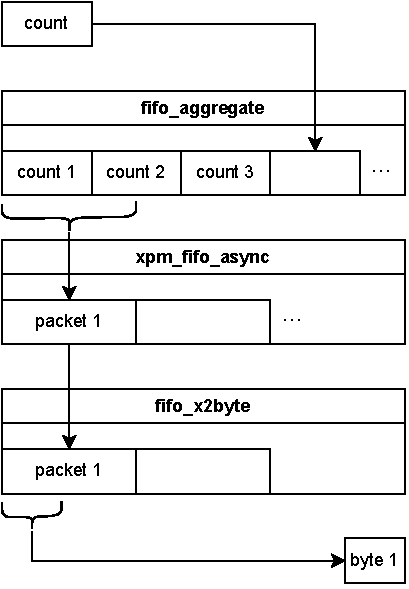
\includegraphics{drawings/fifo_chain.pdf}
    \caption{FIFO chain}
    \label{drw:fifo_chain}
    \vspace{-50pt}
\end{wrapfigure}
The cycle counts determined in the sampling \gls{FSM} are stored in the \gls{BRAM} before being transmitted. The XPM\_FIFO\_ASYNC macro from Xilinx is used to instantiate an asynchronous \gls{FIFO} using the \gls{BRAM} of the \gls{FPGA} \autocite{xilinxVivadoDesignSuite2023}. It supports the usage of different clock signals for data input and output, thus integrating \gls{CDC} functionality. The depth and data read and write width of the \gls{FIFO} are defined as parameters of the macro, with the write depth being limited to values that are a power of two and the data width limited to aspect ratios of 1:1, 1:2, 1:4 and 1:8 for either read or write width. Depending on the write width of the \gls{FIFO}, the available \gls{BRAM} resources can be more or less efficiently used. This is especially relevant because these resources are shared with the \gls{FIFO} of the adc\_driver module.

In order to be more flexible in these terms, a design approach was chosen, in which the results are first aggregated to match the width of the \gls{BRAM} \gls{FIFO} and then passed to said \gls{BRAM} \gls{FIFO} from where they are retrieved and split up into single bytes for transmission. This process is illustrated in \cref{drw:fifo_chain}. The aggregation and splitting logic is implemented in the modules fifo\_aggregate and fifo\_x2byte respectively and described in \cref{sec:helpers}.

\subsection{ADC}
The \gls{ADC} converts the received signal into a 10-bit digital output coded as two's complement. The sampling and conversion rate is determined by the clock provided to the \gls{ADC}, the output latency is 5.5 clock cycles. As the functionality needed for controlling, sampling and transmission is very similar to that of the comparator\_driver shown in the previous section, the following description of the module adc\_driver presents only the significant differences between the modules.

\subsubsection{adc\_driver}
The module adc\_driver has the 10-bit wide signed input (\inlcode{adc_in}) for the parallel output of the \gls{ADC} and outputs \inlcode{adc_en} and \inlcode{clk_adc} for enabling and clocking the \gls{ADC} as well as a \inlcode{trigger_out} signal, which is used by the comparator\_driver module.
The parameters of the module are \inlcode{DEFAULT_POWER}, \inlcode{DEFAULT_TRIG}, \inlcode{DEFAULT_THOLD}, \inlcode{DEFAULT_MAXSMP}, \inlcode{DEFAULT_WIDTH} and \inlcode{DEFAULT_FREQ} along with its respective \inlcode{*_ASCII} representations.

\begin{wrapfigure}{r}{.55\textwidth}
\vspace{-11pt}
\begin{lstlisting}[firstnumber=108,caption={adc\_clkgen instantiation in adc\_driver},label=lst:adc1]
reg [5:0]  freq_state 	= DEFAULT_FREQSTATE;

adc_clkgen  u_adc_clkgen (
	.SSTEP                   ( freq_update  ),
	.STATE                   ( freq_state   ),
	.RST                     ( 1'b0         ),
	.CLKIN                   ( clk          ),
	
	.LOCKED_OUT              ( freq_locked  ),
	.CLK_ADC                 ( clk_adc      )
);
\end{lstlisting}
\vspace{-12pt}
\end{wrapfigure}

Unlike the comparator\_driver, this module uses a variable clock as output to the \gls{FPGA} and for sampling. This functionality allows the user to change the clock frequency in order to either increase the amount of stored data before the \gls{BRAM} \gls{FIFO} is full or to increase the sampling frequency. In order to achieve this, a module named adc\_clkgen is instantiated which receives a signal \inlcode{SSTEP} in order to initiate a frequency change, a 5 bit wide \inlcode{STATE} signal representing the desired frequency, an optional \inlcode{RST} signal and the base clock \inlcode{CLKIN}, from which a clock is synthesized and returned as \inlcode{CLK_ADC} together with a \inlcode{LOCKED_OUT} signal indicating whether the clock is stable. 

The \inlcode{STEP} input is wired to the \inlcode{freq_state} register of the adc\_driver module. Frequencies are selectable in \SI{250}{\kilo\hertz} steps, the lowest being \SI{250}{\kilo\hertz} for the state 0 and the highest being \SI{10}{\mega\hertz} for state 39. The clock synthesis is performed by an instantiation of Xilinx MMCME2\_ADV module, which controls one \gls{MMCM} of the \gls{FPGA} as done by the MMCME2\_BASE module shown in \cref{sec:comp}, but with the option to access its reconfiguration registers by the means of additional input and output signals in order to reconfigure the \gls{MMCM} during runtime. For a correct interfacing and register access, Xilinx provides the module template mmcme2\_drp along with a header file, which were adjusted to define the frequencies for reconfiguration. %TODO Please refer to \cref{sec:mmcme2_drp} for a detailed description of said module.

The input handler \gls{FSM} of adc\_driver accepts a command setting the frequency with the value passed as the desired frequency in kilohertz, e.g. 250. In order to avoid code duplication or division logic, an expanding for-loop has been employed in the respective \inlcode{COMMAND_FREQ} state to compare the number against a possible \inlcode{freq_state} as seen in \cref{lst:adc2} 

\begin{lstlisting}[firstnumber=276,caption={COMMAND\_FREQ state of adc\_driver RX FSM},label=lst:adc2,mathescape=true]
COMMAND_FREQ: begin
	recv_value		 = rx_val;
	recv_value_ascii = 40'h494E56; // "INV"
	
	for (ii = 1; ii <= 40; ii = ii + 1) begin
		if (recv_value == (ii * 250)) begin
			recv_value_ascii	= bin2ascii10000(recv_value);
			
			freq_state			<= ii - 1;
			freq_update			<= 1'b1;
			ascii_val_freq		<= recv_value_ascii;
		end
	end $\lstsetnumber{\ldots}$
    ...$\lstresetnumber\setcounter{lstnumber}{293}$
end
\end{lstlisting}

The sampling \gls{FSM} handles the incoming data in every cycle of set frequency. The \gls{FSM} consists of two states: \inlcode{SAMPLE_RUN} and \inlcode{SAMPLE_RST}. In the \inlcode{SAMPLE_RUN} state, the incoming data is sampled if a triggering is forced manually using the \inlcode{force_single} register, the (simulated) input exceeds the value  of the \inlcode{trigger_threshold} register while triggering is enabled (\inlcode{trigger} register) or if the sampling was already triggered and is not yet finished as indicated by the \inlcode{triggered} register. The sample is shifted such, that the in register \inlcode{width} specified number of bits are written to the \inlcode{sample_in} register which feeds the input \gls{FIFO}. While the input \gls{FIFO} takes inputs of the width \inlcode{MAX_SAMPLE_WIDTH}, only an adjustable number defined by said \inlcode{width} register are stored.

If the \gls{BRAM} \gls{FIFO} is full or \inlcode{sample_count} reached 0, the sampling is stopped and the \gls{FSM} continues to the \inlcode{SAMPLE_RST} state, which waits until the transmission logic applies a reset signal. As that reset signal is set for only one cycle in the faster system clock domain, it is stretched before being synchronized to the \inlcode{clk_adc} using the module pulse\_stretcher so that the pulse is not missed. The resulting signal is named \inlcode{reset_w_extd_adc}.

\begin{lstlisting}[firstnumber=477,caption={SAMPLE\_RUN state of adc\_driver sampling FSM},label=lst:adc3]
// Run state: trigger on force signal or when threshold is exceeded
// 			  write samples to infifo and keep triggered until sample_count is reached or bram is full
SAMPLE_RUN: begin
	if (force_single_adc || 
		(trigger_adc && adc_in > trigger_threshold_adc && !sim_switch_adc) || 
		(trigger_adc && sim_adc_in > trigger_threshold_adc && sim_switch_adc) || 
		triggered) begin
			if (sample_count > 0 && !bram_full) begin
				if (sim_switch_adc)
					sample_in		<= sim_adc_in >> (MAX_SAMPLE_WIDTH - width_adc);
				else
					sample_in		<= adc_in >> (MAX_SAMPLE_WIDTH - width_adc);
				sample_in_vld	<= 1'b1;
				triggered 		<= 1'b1;
				sample_count	<= sample_count - 1;
			end
			else begin
				sample_in_vld	<= 1'b0;
				triggered 		<= 1'b0;
				sample_count	<= 1'b0;
				state_sample	<= SAMPLE_RST;
			end
	end
	else begin
			sample_in_vld		<= 1'b0;
	end
end
\end{lstlisting}

The adc\_driver module also employs logic for outputting a trigger signal. This output \inlcode{trigger_out} is always '1' if \inlcode{adc_in} exceeds the threshold and is synchronous to \inlcode{clk_adc}.

\begin{lstlisting}[firstnumber=531,caption={trigger\_out process of adc\_driver},label=lst:adc4]
always @(posedge clk_adc) begin
	if (adc_in >= trigger_threshold_adc && !sim_switch_adc ||
		sim_adc_in >= trigger_threshold_adc && sim_switch_adc)
			trigger_out_adc <= 1;
	else
			trigger_out_adc <= 0;
end
\end{lstlisting}
The simulation logic emulates a input which is incremented by 1 each \inlcode{clk_adc} clock cycle.


\subsection{Piezo driver}\label{sec:commlogic}
The logic for driving the piezo is defined within the module piezo\_driver which is instantiated and controlled by its instantiating module comm\_protocol. The comm\_protocol receives commands from the host or button inputs and directs the piezo\_driver to switch the low and high input of the gate driver and consequently the half-bridge driving the piezo. The transmission of the digital code is performed using \gls{OOK} modulation scheme, which represents digital data by a defined duration of presence or absence of a carrier wave \autocite{maximintegratedOOKYouRe2009}. 

\subsubsection{comm\_protocol}
The module comm\_protocol has a single input \inlcode{button_start} and outputs a signal \inlcode{comm_fin} and the signals for switching the gate driver inputs (\inlcode{piezodriver_hi} and \inlcode{piezodriver_lo}). Additionally it communicates with the serial\_interface module to receive and transmit data. The parameters of the module mainly set the default pulsing durations for charging (\inlcode{DEFAULT_CHP}),  a '0' bit (\inlcode{DEFAULT_0L}), a '1' bit (\inlcode{DEFAULT_1L}) and the break durations in microseconds before starting a transmission (\inlcode{DEFAULT_STL}) and in between the pulses (\inlcode{DEFAULT_BRL}). The parameter \inlcode{DEFAULT_DATA} sets the 4 default bits to be transmitted and \inlcode{DEFAULT_CLKDIV} sets the default clock divider to create the frequency with which the piezo is being switched. As for the other modules, the default values can be changed using the \gls{UART} interface.

\begin{wrapfigure}{r}{.6\textwidth}
\begin{lstlisting}[firstnumber=78,caption={piezo\_driver and delay instantiation in comm\_protocol},label=lst:comm1]
reg [11:0] piezo_numpulses	= 0;
reg [8:0] piezo_clkdiv		= DEFAULT_CLKDIV;
wire [21:0] piezo_start_cfg	= {piezo_clkdiv, piezo_numpulses, piezo_start};

//wire piezo_start_100, piezo_fin_100;
wire piezo_start_cfg_rcv, piezo_fin, delay_fin;

piezo_driver m_piezo_driver (
	.clk                (clk),
	.start_cfg          (piezo_start_cfg),
	.start_cfg_rdy      (piezo_start_cfg_rdy),
	.start_cfg_rcv      (piezo_start_cfg_rcv),
	.fin                (piezo_fin),
	.piezodriver_lo     (piezodriver_lo),
	.piezodriver_hi     (piezodriver_hi)
);

delay m_delay (
	.clk_12             (clk),
	.delay_us           (delay_us),
	.start              (delay_start),
	.fin                (delay_fin)
);
\end{lstlisting}
\vspace{-20pt}
\end{wrapfigure}
As mentioned before, the module instantiates piezo\_driver in order to determine the pulse frequency and the number of pulses the piezo is supposed to generate. The \inlcode{piezo_start_cfg} wire combines the signals \inlcode{piezo_clkdiv}, \inlcode{piezo_numpulses} and \inlcode{piezo_start} and passes it to the module together with the \inlcode{piezo_start_cfg_rdy} signal. The module returns whether it received the config and excecuted the pulsing operation to \inlcode{piezo_start_cfg_rcv} and \inlcode{piezo_fin} respectively. The implementation of the module is described further below.
The delay module takes \inlcode{delay_us} and \inlcode{delay_start} as inputs and returns '1' to \inlcode{delay_fin} if the internal counter reaches the value specified in \inlcode{delay_us}. This counter is only incremented every 12 system clock cycles, which equals one microsecond.

The main part of the comm\_protocol is the communication \gls{FSM}, which defines the communication pattern. The \gls{FSM} starts with state 0, sensing for \inlcode{comm_start} which is either enabled by button or by its respective command. if the register is high, \inlcode{comm_fin} is unset and the \gls{FSM} continues to the next state. State 1 sets \inlcode{piezo_numpulses} to the \inlcode{Charge_Pulses} register and sets \inlcode{piezo_start} to high. State 2 unsets these signals if peizo\_driver received the signals. States 3 and 4 set and unset \inlcode{delay_start}. This pattern continues with the transmission of the defined pattern of '0' and '1' bits and the defined break in between until all 4 bits have been transmitted.

An additional testing \gls{FSM} has been implemented which simply repeats the tranmsission of the \inlcode{Charge_Pulses} without breaks in between, resulting in a constant transmission. The test state is either initiated with the respective serial command or with \inlcode{button_start} if the module was synthesized with a \inlcode{COMM_TEST} flag defined within the module.

\subsubsection{piezo\_driver}
The piezo\_driver module synthesizes a \SI{250}{\mega\hertz} clock with the Xilinx MMCME2\_BASE module, which is divided down to a desired frequency using the value defined in \inlcode{piezo_clkdiv} of comm\_protocol.
To achieve this, the received \inlcode{start_cfg} is synchronized to the \inlcode{clk_250} clock. The clock and state control \gls{FSM} senses for the \inlcode{start} register in state \inlcode{IDLE} and continues to state \inlcode{BUSY} if it is set. State \inlcode{BUSY} increments \inlcode{clk_counter} until \inlcode{counter_compare_value} is reached, which is set to the value of \inlcode{piezo_clkdiv}. If it is reached, the \gls{FSM} is in the state \inlcode{BUSYPULSE} for one cycle, where the \inlcode{pulse_counter} register is incremented by one and which either continues with state \inlcode{IDLE} if the \inlcode{pulse_counter} reached \inlcode{numpulses} or otherwise returns to state \inlcode{BUSY}.

\begin{wrapfigure}{r}{.5\textwidth}
\begin{lstlisting}[firstnumber=110,caption={Snippet of MOSFET output FSM of piezo\_driver},label=lst:comm2]
OUT1_WAIT : begin
    dly0 <= DLY;
    out0 <= 0;

    dly1 <= dly1 - 1;
    out1 <= 0;
    if (dly1 == 0)
        state_out <= OUT1;
end
OUT1 : begin
    out1 <= 1;
    if (state == BUSYPULSE)
        state_out <= OUT0_WAIT;
end
\end{lstlisting}
\vspace{-20pt}
\end{wrapfigure}
The \gls{MOSFET} output \gls{FSM} senses in which state the clock and state control \gls{FSM} is and cycles though its own states \inlcode{state_out} accordingly. In \inlcode{state_out IDLE}, both outputs \inlcode{out0} and \inlcode{out1} are set to '0'. If the other \inlcode{state} changes to \inlcode{BUSY}, \inlcode{state_out} continues to \inlcode{OUT1_WAIT}. This wait state sets both output signals to '0' and is responsible for providing the delay in order to avoid shoot-throughs as described in \cref{sec:driverschem}. If \inlcode{dly1} reached 0 after decrementing in each clock cycle, the \gls{FSM} proceeds to \inlcode{state_out OUT1}, in which \inlcode{out1} is set to '1', as seen in \cref{lst:comm2}. This changes only after a \inlcode{BUSYPULSE} as the \inlcode{state_out OUT0_WAIT} is entered thereafter and both output signals are set to '0'. The \inlcode{state_out OUT0} acts in the same manner as \inlcode{OUT1} and is therefore not further described. Independant of the current \inlcode{state_out}, the \gls{FSM} switches to \inlcode{state_out IDLE} if \inlcode{state} is \inlcode{IDLE}.

The outputs \inlcode{out0} and \inlcode{out1} are assigned to \inlcode{piezodriver_lo} and \inlcode{piezodriver_hi} respectively.

\subsection{Helpers}\label{sec:helpers}
Multiple modules mentioned in the previous sections instantiated the modules fifo\_aggregate, fifo\_x2byte and/or mmcme2\_drp. As they are more complex, the former two are described within this section for a better understanding. Please refer to the in-file documentation for changing mmcme2\_drp.

\subsubsection{fifo\_aggregate}
The module fifo\_aggregate has the purpose to store an input of adjustable width in order to aggregate it and return it as an output of higher width. For that purpose it has \inlcode{rst}, \inlcode{input_width} and \inlcode{wr_en} as inputs and outputs \inlcode{data_out} and \inlcode{full}. The module has the parameters \inlcode{MAX_INPUT_WIDTH} and \inlcode{OUTPUT_WIDTH_BYTES} which define the maximum input width and the actual output width respectively.

As the output width may not be a perfect multiple of the input, the modules shift register width is the output width plus the maximum input width.
The shift register is shifted by a variable amount of bits each time a \inlcode{wr_en} is applied. 

If the current written bit count \inlcode{counter} plus \inlcode{input_width} does not exceed \inlcode{OUTPUT_WIDTH}, \inlcode{current_shift_amount} is set to \inlcode{input_width} + \inlcode{overflow}. This \inlcode{overflow} register differs from 0 only if \inlcode{OUTPUT_WIDTH} is exceeded during a write to the \gls{FIFO}. In the case that \inlcode{counter} plus \inlcode{input_width} reaches or exceeds \inlcode{OUTPUT_WIDTH}, the \inlcode{current_shift_amount} is set to the number of remaining bits until it is full and the number of remaining bits is stored in \inlcode{current_overflow} in order to be shifted in the next clock cycle. Additionally \inlcode{full} is set to '1' indicating a valid output. 

The shift register right shifts according to \inlcode{current_shift_amount} and inserts the arriving bits according to \inlcode{input_width} and \inlcode{current_overflow} to the left of the existing data.

\subsubsection{fifo\_x2byte}
The module fifo\_x2byte has the purpose to split data input with the width of multiple bytes to a single byte output. It receives \inlcode{rst}, \inlcode{rd_en}, \inlcode{wr_en} and \inlcode{data_in} as inputs and returns \inlcode{data_out} and the status registers \inlcode{full} and \inlcode{empty}.
The width of the input is defined by the module parameter \inlcode{INPUT_WIDTH_BYTES}, the parameter \inlcode{FIFO_DEPTH_INPUT} defines the number of stored inputs.

The module employs a common \gls{FIFO} pattern with seperate read and write pointers. The memory is an 8-bit vector array with a depth of \inlcode{MAX_NUM_BYTES} (= \inlcode{INPUT_WIDTH_BYTES * FIFO_DEPTH_INPUT}). If an input is stored, \inlcode{wr_ptr} is either increased by \inlcode{INPUT_WIDTH_BYTES} or its \gls{MSB} is inverted and the other bits set to '0' if the \inlcode{wr_ptr} would reach \inlcode{MAX_NUM_BYTES} otherwise. This \gls{MSB} enables checking, whether the \gls{FIFO} is full (if the write and read pointers have a different \gls{MSB}) or empty (otherwise). The \inlcode{full} flag is checked before storing an input.

If \inlcode{rd_en} is set to '1' and the \gls{FIFO} is not empty, the read pointer is either incremented by 1, or its MSB is inverted and the other bits are set to '0', if it would reach \inlcode{MAX_NUM_BYTES}, analog to the behaviour of the \inlcode{wr_ptr}.

The output \inlcode{data_out} is assigned to \inlcode{memory[rd_addr]}, with \inlcode{rd_addr} being \inlcode{rd_ptr} without its \gls{MSB}, making the \gls{FIFO} first-word-fall-through (FWFT), as the output is available without latency.

%\subsubsection{mmcme2\_drp}\label{sec:mmcme2_drp}
%The module mmcme2\_drp provides the signaling 


\chapter{Results \& Discussion}\label{chap:results}
This chapter evaluates the implementation in consideration of the objectives laid out in \cref{sec:overview}. This includes mainly the actual ultrasonic communication but also extends to the parts of software and hardware enabling the functionality. For the transmission tests, a SONOSCAN RMC 2.25 piezoelectric transducer (A) with a resonance frequency of around \SI{2.09}{\mega\hertz} has been used, which is tightly pressed against a steel beam in an angle of 60° using a mount, magnets and ultrasound gel. As one piezo element failed during a thermal stress test, the reception tests used two not further specified piezoelectric transducers (B) with a resonance frequency of around \SI{121}{\kilo\hertz}. These are put in a metal enclosure in a 90° angle. All test articles can be seen in \cref{img:versuchsaufbau}.

\begin{figure}[H]
    \centering
    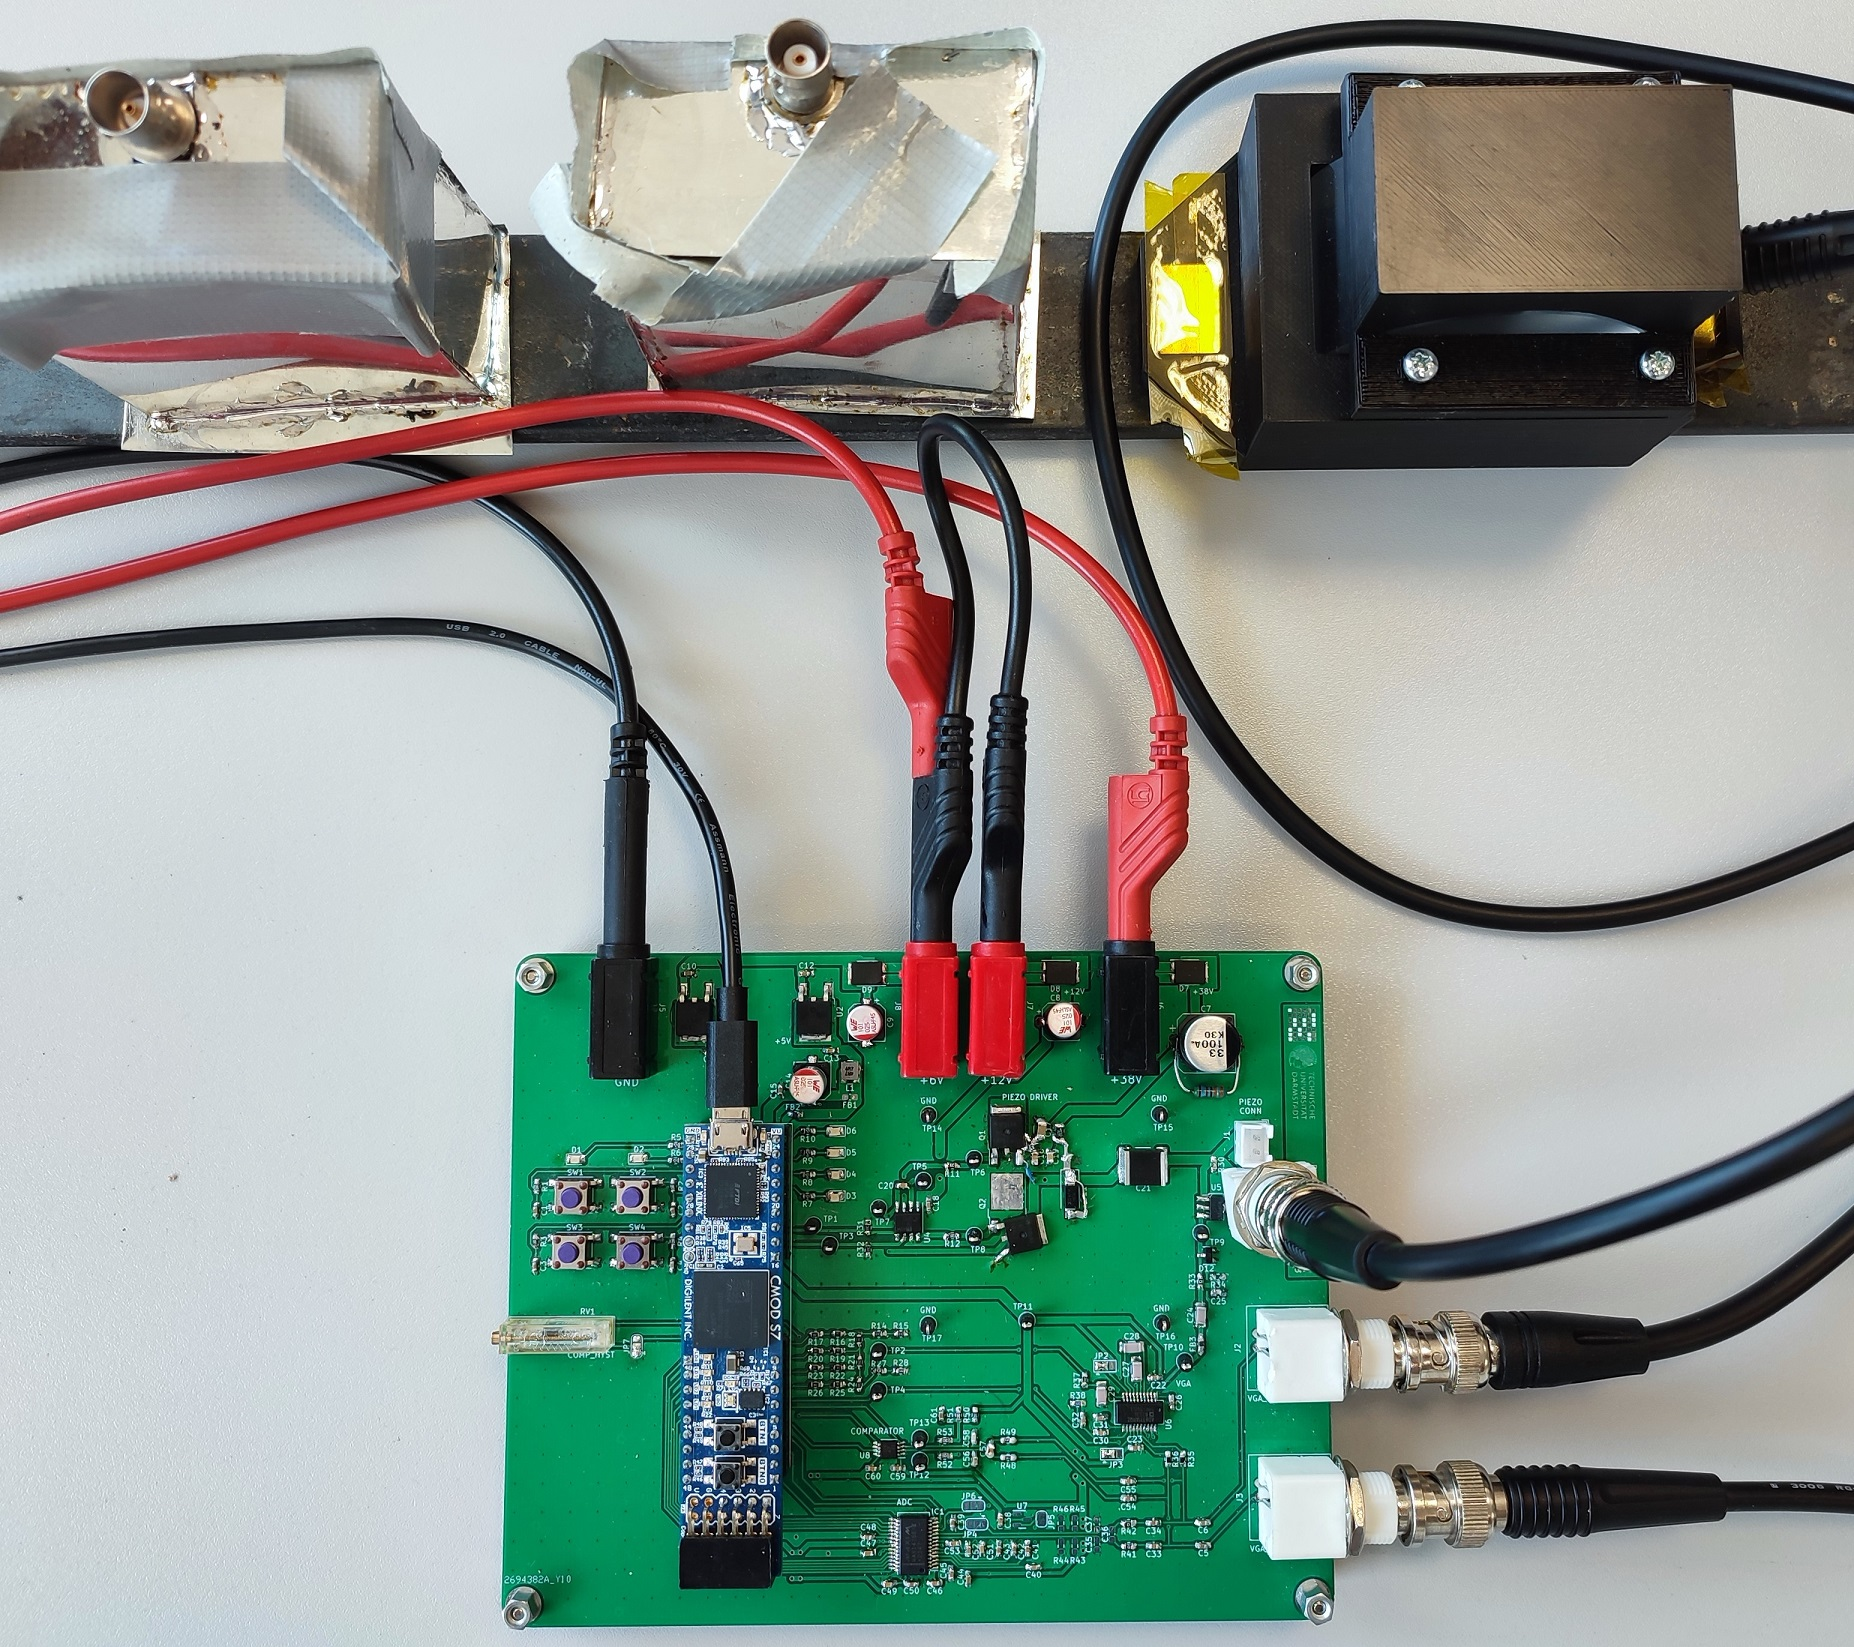
\includegraphics[width=0.8\columnwidth]{images/versuchsaufbau2.jpg}
    \caption{All test articles: PCB, two unspecified piezos (A) in a metal enclosure, single SONOSCAN piezo (B)}
    \label{img:versuchsaufbau}
\end{figure}

\section{Ultrasonic transmission}
The ultrasonic transmission is in terms of hardware enabled by the \glsreset{VCVS}\gls{VCVS} consisting of the \gls{MOSFET} gate driver and the \gls{MOSFET} half-bridge and in terms of software by the logic defined in the Verilog module comm\_protocol with its instance of piezo\_driver. To decrease ringing for the targeted transducer (A), two snubber capacitors with $C_{snub} = \SI{15}{\pico\farad}$ have been soldered between drain and source of both half-bridge \glspl{MOSFET} according to the methodology shown in \autocite{johnbettenPowerTipsCalculate2016} and as verified in tests. This dampens the otherwise present ringing overshoots with frequencies of around \SI{150}{\mega\hertz}.

The default parameters have been set such, that a the bit pattern '0101' should be transmitted with a clock divider value of 200. This should result in a \SI{625}{\kilo\hertz} switching frequency for the piezo element.

\Cref{img:piezo_unbelastet1} shows the signals applied to the gate driver and the unterminated signal at the BNC connector output to the piezo transducer.  The frequency matches the targeted \SI{625}{\kilo\hertz}.
The transmission procedure is performed as desired with first transmitting the charging pulses, then waiting the defined start timeout and finally sending the four bits consecutively with the defined break timeouts in between. The bit pattern matches the pattern defined in the module. The timeouts are defined in microseconds and are by default \SI{500}{\micro\s} after the charging pulse and \SI{100}{\micro\s} after each bit. The pulses are for testing a count of 100 for charging, 100 for a '0' and 200 for a '1'. The measurements show, that the the count is correct as $\SI{625}{\mega\hertz}\cdot\SI{320}{\micro\s} = 200$ cycles.
As can be seen in \cref{img:piezo_unbelastet2}, the signal is not substantially delayed and the pulse width is uniformly half the clocking cycle.

\begin{figure}[H]
    \centering
    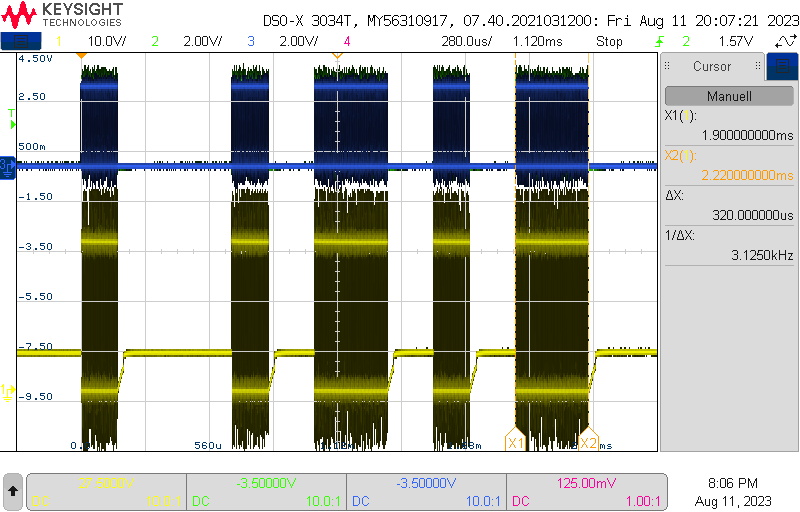
\includegraphics[width=0.8\columnwidth]{images/piezo_unbelastet1.png}
    \caption{Packet waveform of unloaded transmission; channel 1: output of the MOSFET half-bridge, channels 2 \& 3: low-side and high-side signals from the FPGA}
    \label{img:piezo_unbelastet1}
\end{figure}
\begin{figure}[H]
    \centering
    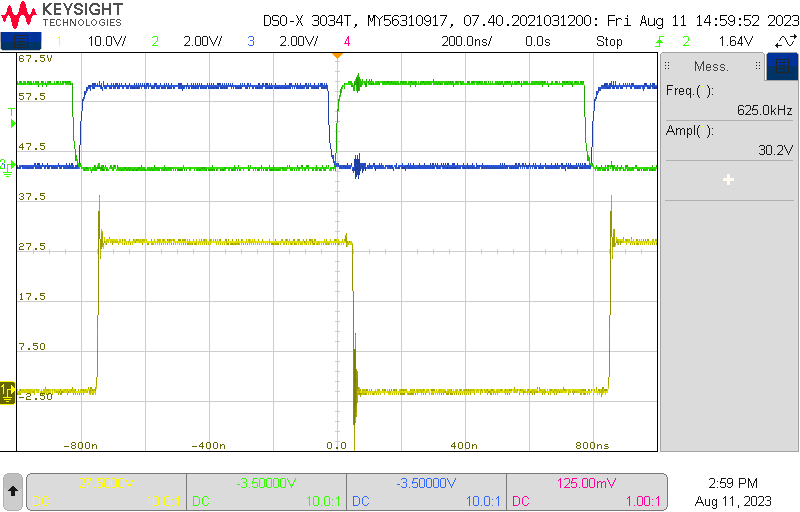
\includegraphics[width=0.8\columnwidth]{images/piezo_unbelastet2.png}
    \caption{Detailed waveform of unloaded transmission; channel 1: output of the MOSFET half-bridge, channels 2 \& 3: low-side and high-side signals from the FPGA}
    \label{img:piezo_unbelastet2}
\end{figure}

For the next test, the piezo element (A) has been connected to the BNC connector. The clock divider has been set to 60 for a pulsing frequency of around \SI{2}{\mega\hertz}. Reception could be verified using its counterpart before its destruction, although images can't be provided.

Instead, piezo transucers (B) were used at a transmission frequency of \SI{313.3}{\kilo\hertz}, as the dominant resonance frequency of \SI{121}{\kilo\hertz} can't be achieved with the boundaries of the clock divider. \Cref{img:piezo_belastet4} shows the received signal at the secondary piezo element connected to the oscilloscope. Its Fourier transform reveals that the power is highest at around \SI{313}{\kilo\hertz} confirming a successful transmission.

As can be seen, the requirements for data transmission are met. Commands passed to the comm\_protocol module are interpreted correctly and the frequency is changed as desired. The \gls{PCB} is able to drive a piezo transducer with frequencies over \SI{2}{\mega\hertz} with a sustained average current of \SI{400}{\milli\ampere} as verified in a stress test. The tests were able to show the communication pattern which was defined by the original version of the code. Due to the addition of an adjustable clock divider, transmission using frequency modulation is also feasible with a low effort for code rewrite.


\begin{figure}[H]
    \centering
    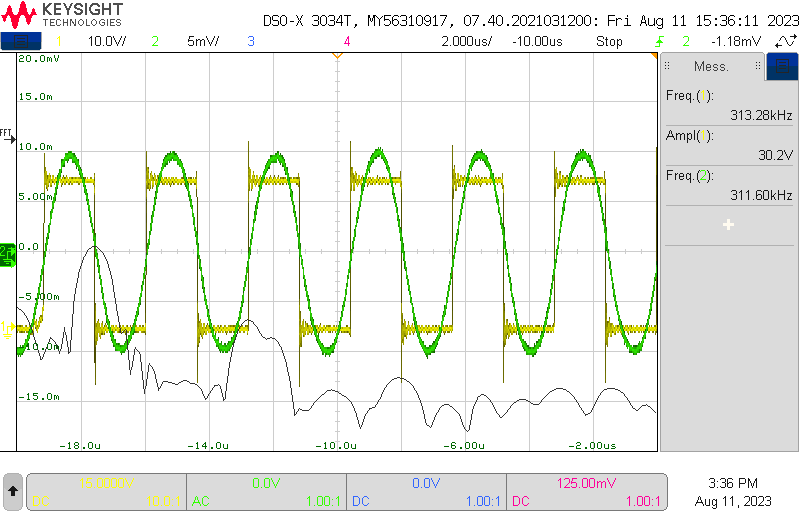
\includegraphics[width=0.8\columnwidth]{images/piezo_belastet4.png}
    \caption{Waveform of transmission with a piezo (B) as load; channel 1: output of the MOSFET half-bridge, channel 2: signal generated by receiving piezo}
    \label{img:piezo_belastet4}
\end{figure}

\section{Ultrasonic reception}
The reception and processing of ultrasonic signals is in terms of hardware mainly enabled by the \gls{LNA}, the \gls{ADC} and the comparator and in terms of software by the modules vga\_driver, adc\_driver and comp\_driver along its instantiated modules.

For the first test, a signal generator was connected to the BNC connector and set up to generate a sine wave with a frequency of \SI{2}{\mega\hertz} and an amplitude of \SI{10}{\milli\volt}. \Cref{img:piezo_inbnc1} shows the differential output of the \gls{VGA}. The output is taken from the BNC connectors connected to the oscilloscope with enabled AC coupling.
The gain of the \gls{VGA} is set to '1111' using the buttons. As seen, the amplified signal is not shifted compared to the source. This would not be a concern however, as there is no need to be in phase with the source, either way the digitization with the \gls{ADC} shifts the signal due to its 5.5 system clock cycle latency. The amplification matches the expected \SI{43}{\decibel} of the \gls{VGA} (LO gain mode) and the signal keeps its shape.
\begin{figure}[h]
    \centering
    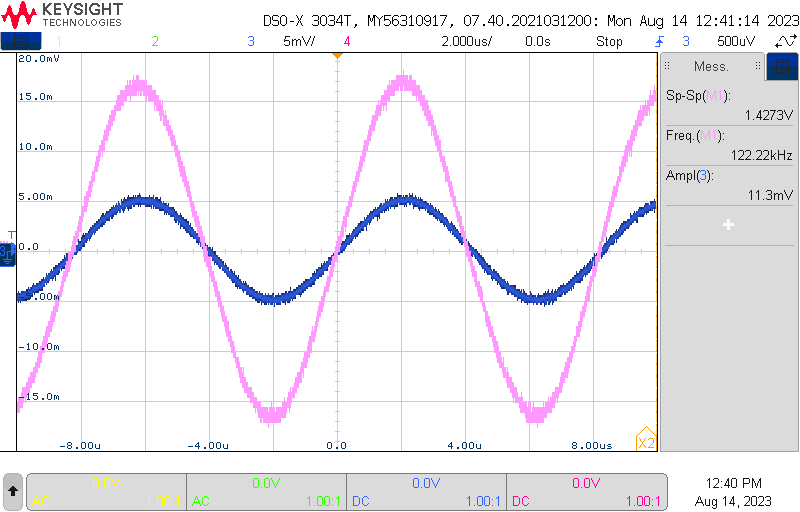
\includegraphics[width=0.8\columnwidth]{images/piezo_vga.png}
    \caption{Waveform of VGA output; channel 3: output of the signal generator, pink waveform: differential VGA\_OUT}
    \label{img:piezo_inbnc1}
\end{figure}
%TODO: new pic
One potential issue that became apparent during later \gls{ADC} testing is that the gain increases linearly on a logarithmic scale. That means a binary gain setting of 8 amplifies the signal by a factor of 10 (\SI{20}{\decibel}) whereas a setting of 14 gives a factor of nearly 100 (\SI{40}{\decibel}). Depending on the signal range this can be desired, but it should be considered. Because of this, a more precise \gls{DAC} would greatly enhance the gain setting.

For a more realistic testing, the signal generator has been connected to the secondary piezo element (B) and set up to generate a sine wave at the resonance frequency of \SI{121}{\kilo\hertz} with an amplitude of \SI{5}{\volt} for the following tests. The primary piezo (B) is connected to the BNC connector of the \gls{PCB}.

Testing the comparator, \cref{img:piezo_comp} shows the amplified differential signal as well as the output signal of the comparator, sampled by the oscilloscope using a passive probe. The comparator output follows the received and amplified signal closely. A small phase shift exists which is mainly due to the hysteresis setting, but the duration of the positive and negative half wave matches the pulse width of the comparator output.
\begin{figure}[h]
    \centering
    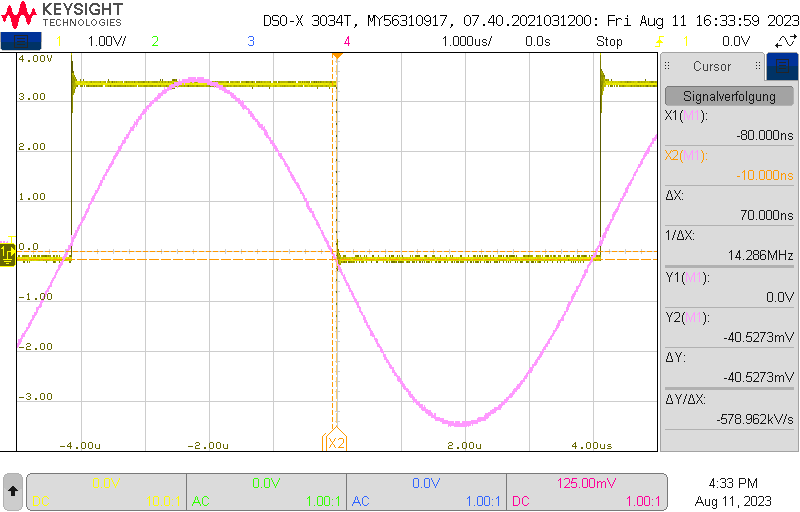
\includegraphics[width=0.8\columnwidth]{images/piezo_comp1.png}
    \caption{Waveform of comparator output; channel 1: output of the comparator, pink waveform: differential VGA\_OUT}
    \label{img:piezo_comp}
\end{figure}


\begin{wraptable}{r}{0.35\textwidth}
\centering
\subfloat[comparator]{
\begin{tabular}{||c|c||}
\hline
\SI{121}{\kilo\hertz} & \SI{122}{\kilo\hertz} \\
\hline\hline
207 & 205 \\
207 & 205 \\
206 & 204 \\
207 & 205 \\
206 & 205 \\
207 & 206 \\
207 & 204 \\
206 & 205 \\
207 & 205 \\
206 & 205 \\
207 & 205 \\
207 & 205 \\
\hline
\end{tabular}
}
\subfloat[ADC]{
\begin{tabular}{||c||}
\hline
\SI{121}{\kilo\hertz} \\
\hline\hline
-224    \\
-213    \\
-188    \\
-152    \\
-106    \\
-54     \\
2       \\
57      \\
109     \\
153     \\
187     \\
208     \\
\hline
\end{tabular}
}
\caption{Sampling excerpts}
\label{tab:samples}
\vspace{-15pt}
\end{wraptable}

The comparator\_driver module samples the comparator output at \SI{50}{\mega\hertz}, counts the number of cycles for a signal switch and streams the data to an external computer. The left column of \cref{tab:samples}a shows an excerpt of the output of the comparator after the bitstream has been converted to a readable format using a self-written Python script. As the values only show the clock cycles for a half-wave, two values have to be added in order to get the actual number of cycles for a complete signal period. The formula $f_{signal}=\frac{\SI{50}{\mega\hertz}}{num\_cycles_{lo\_hi} + num\_cycles_{hi\_lo}}$ yields $f_{signal}=\SI{120.985}{\kilo\hertz}$ averaged over the shown excerpt, matching the frequency set at the function generator. The right column of \cref{tab:samples}a shows an excerpt when the clock is increased by \SI{1}{\kilo\hertz}, showing a difference of 4 cycles on average for a signal period.


The \gls{ADC} testing was performed by triggering on a threshold, with a sampling frequency of \SI{3}{\mega\hertz}, a sampling width of 10 bits and a sampling length of 40000 samples.
As the output clamping level has been set such, that $V_{pp,diff} = \SI{2.5}{\volt}$, the \gls{ADC} currently does not make use of its full \SI{\pm4}{\volt} input range and is thus limited in resolution. In order to maximize the \gls{SNR}, the \SI{10}{\kilo\ohm} $R_{clmp}$ resistor (R38) should be removed, as the differential peak-to-peak voltage is clamped to $V_{pp}=\SI{4.5}{\volt}$ by the \gls{VGA} anyway, eliminating the need for additional protection for the \gls{ADC} and comparator.

\Cref{tab:samples}b shows an excerpt of the sampled integer values for a \SI{121}{\kilo\hertz} signal received from the piezo (B) and amplified to a differential peak-to-peak voltage of approximately $V_{pp,diff}=\SI{1.75}{\volt}$, measured using the VGA\_OUT+ and VGA\_OUT- connectors.
This should lead to sample values in the range of  $\pm\frac{\SI{1.75}{\volt}}{\SI{4}{\volt}} * 1024 / 2 = \pm224$, which can be confirmed by the received results. \Cref{fig:adc_signal_time} shows the sinusoidal signal reconstructed from the samples, while \cref{fig:adc_signal_freq} shows the respective Fourier transform.
% \begin{figure}[H]
% \centering
% \begin{minipage}{.5\textwidth}
%   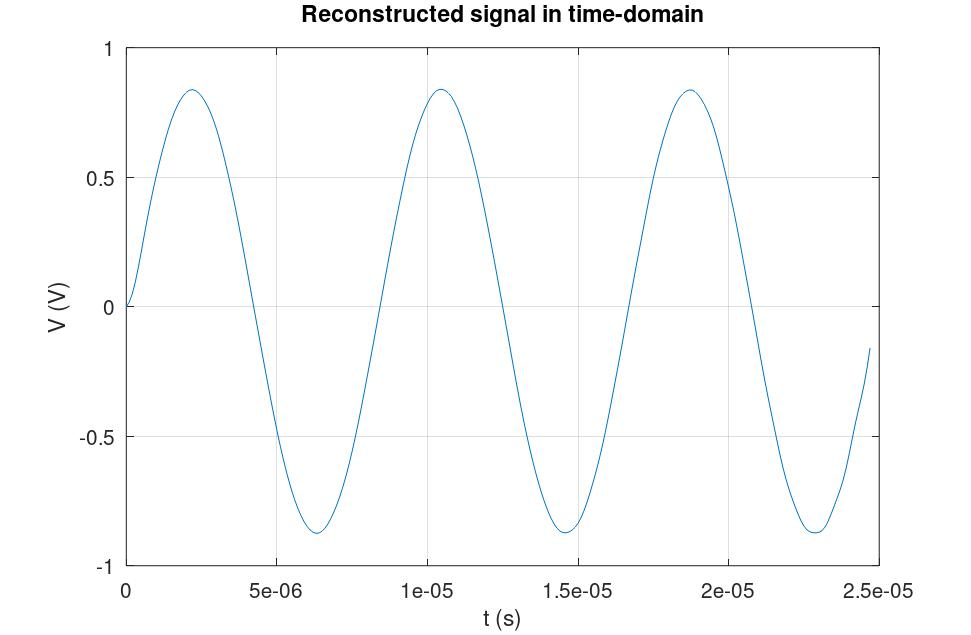
\includegraphics[width=\linewidth]{images/adc_121_time.jpg}
%   \captionof{figure}{Reconstructed signal in time domain}
%   \label{fig:adc_signal_time}
% \end{minipage}%
% \begin{minipage}{.5\textwidth}
%   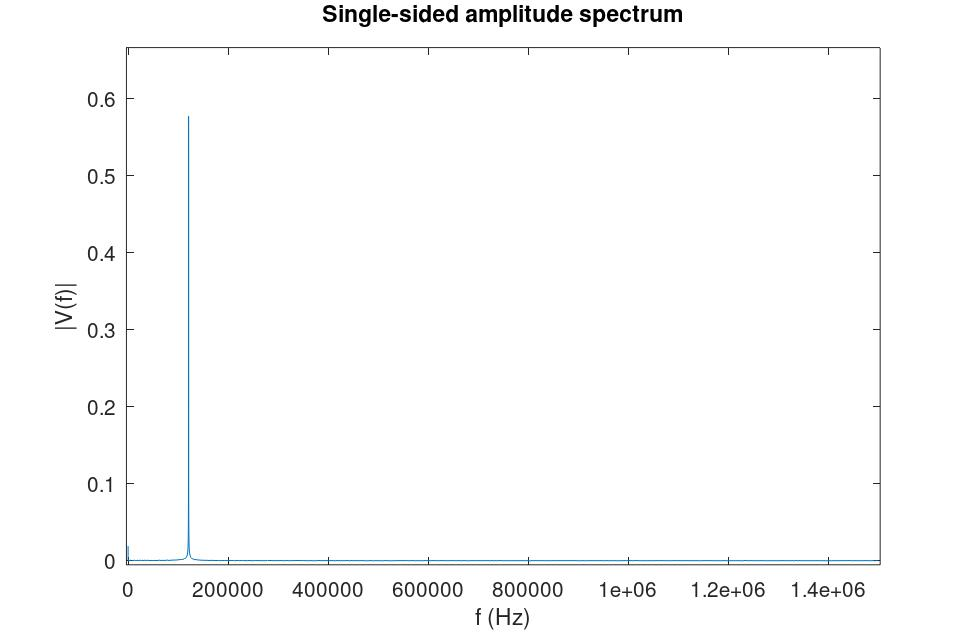
\includegraphics[width=\linewidth]{images/adc_121_fft.jpg}
%   \captionof{figure}{Fourier transform of sampled signal}
%   \label{fig:adc_signal_freq}
% \end{minipage}
% \end{figure}

\begin{figure}
    \centering
    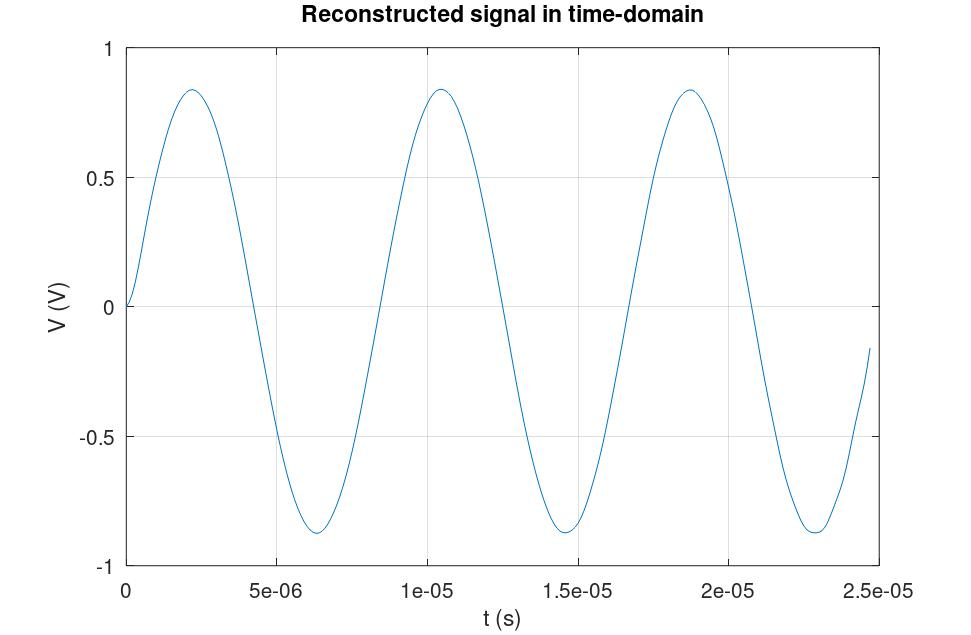
\includegraphics[width=0.8\columnwidth]{images/adc_121_time.jpg}
    \caption{Reconstructed signal in time domain}
    \label{fig:adc_signal_time}
\end{figure}
\begin{figure}
    \centering
    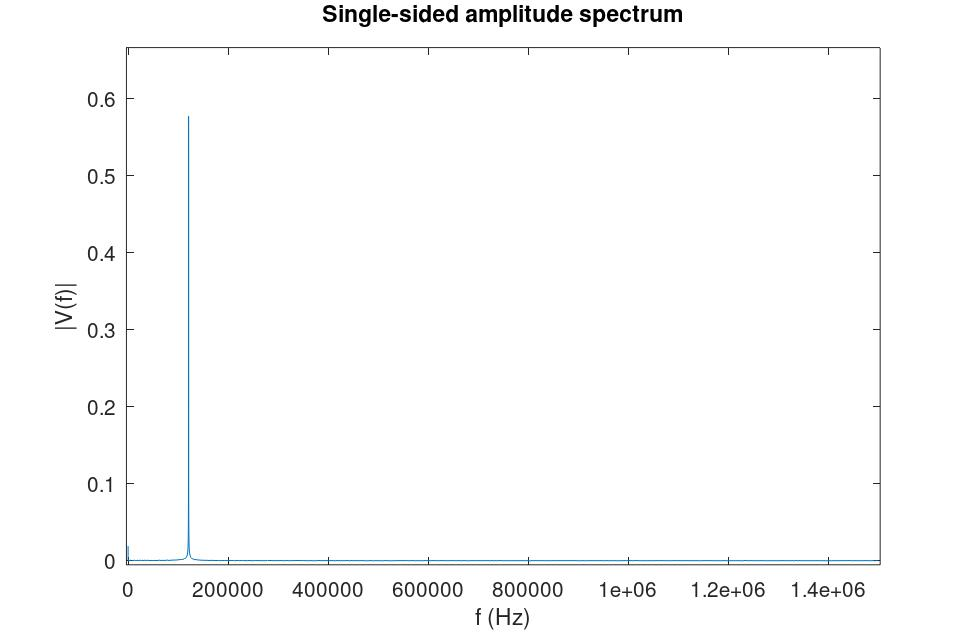
\includegraphics[width=0.8\columnwidth]{images/adc_121_fft.jpg}
    \caption{Fourier transform of sampled signal}
    \label{fig:adc_signal_freq}
\end{figure}
%TODO cref listing



\section{PCB design}
The PCB design uses a standard two layer stackup and was manufactured by JLCPCB. Before manufacturing, electrical rule checking (ERC) as well as design rule checking (DRC) was performed in order to verify the pin connections of the schematic as well as the design rules and schematic parity of the \gls{PCB} layout. The only major issue within the first design was an incorrect pin order of the half-bridge \glspl{MOSFET}. For testing purposes, this issue could be fixed manually by some sanding and the use of a single flying wire. The schematic and layout shown in \cref{chap:impl} show a fixed second iteration of the \gls{PCB} schematic and layout. Other minor improvements of the second iteration are the increased footprint size of the \gls{LDO} input and output capacitors, the addition of a BNC connector footprint and more footprints for the possibility of a more complex passive filter network at the \gls{ADC} and comparator. A third iteration with additional footprints for an optional R-C snubber, further improved footprint sizes and capacitor discharge resistors has been uploaded to the project, but could not be reflected in the schematics of the report.

\section{FPGA logic}
The \gls{FPGA} logic was written in Verilog using Xilinx macros for clock generation, clock domain crossing and \gls{BRAM} instantiation. All modules have been tested with the use of behavioral testbench simulations in Vivado and by examining the behavior when deployed to the \gls{FPGA} and used for ultrasonic communication.

For easy usage without a host computer, the latest version of the implemented bitstream has been exported as a bin file and stored on the flash memory of the \gls{FPGA}, such that it is loaded when powered on.

\subsubsection{Serial communication}

Most of the functionality is initiated by commands sent over the serial interface. \Cref{lst:serdef1} shows the available commands as defined in serial\_defines.hv. The serial interface works robustly and offers a convenient command structure. In order to add additional commands or to interface additional modules, only few changes in code are needed. 
\begin{lstlisting}[caption={Command strings as defined in serials.hv},label=lst:serdef1]
// command structure: "DESTINATION:COMMAND VALUE\n"
// e.g.                      "VGA:GAIN 1\n"

/*  Available Commands:
// VGA:POWER [0/1]: enables/disables vga.
// VGA:STATUS [<any number>]: return status message.
// VGA:GAIN [0..15]: sets the vga gain.
// VGA:RESET [<any number>]: resets signals

// COMM:START [<any number>]: starts the communication protocol with defined settings and data.
// COMM:TEST [0/1]: enables/disables the communication test state.
// COMM:STATUS [<any number>]: return status message.
// COMM:SETDTA [0..15]: sets the transmission data.
// COMM:SETCHP [0..4095]: sets the amount of charge pulses.
// COMM:SETSTL [0..65535]: sets the start delay in microseconds.
// COMM:SET0L [0..4095]: sets the amount of pulses for a 'zero' bit.
// COMM:SET1L [0..4095]: sets the amount of pulses for a 'one' bit.
// COMM:SETBRL [0..65535]: sets the break delay in microseconds.
// COMM:CLKDIV [0..511]: sets the piezo clock divider value.
// COMP:RESET [<any number>]: resets signals

// ADC:POWER [0/1]: enables/disables adc.
// ADC:STATUS [<any number>]: return status message.
// ADC:TRIG [0/1]: enable triggering according to threshold.
// ADC:THOLD [0..1023]: set threshold. IMPORTANT: signed number -> values >511 are negative.
// ADC:MAXSMP [0..65535]: set maximum amount of samples. '0' equals maximum samples (18'd262.143).
// ADC:FORCE [<any number>]: force immediate triggering.
// ADC:FREQ [250..10000]: sets sampling frequency in kHz if input is valid. steps of 250 kHz.
// ADC:WIDTH [0..10]: sets sampling width.  
// ADC:RESET [<any number>]: resets signals (TODO) and applies reset (emptiing fifos)
// ADC:SIM [0/1]: use simulation data instead of adc_in pins input

// COMP:POWER [0/1]: enables/disables comp.
// COMP:STATUS [<any number>]: return status message.
// COMP:MAXSMP [0..65535]: set maximum amount of samples. '0' equals maximum samples (18'd262.143).
// COMP:TRIG [0/1]: enable triggering according to adc threshold.
// COMP:FORCE [<any number>]: force immediate triggering.
// COMP:FREQ [25/50/100/200/300/400]: sets sampling frequency in MHz if input is valid. CURRENTLY REMOVED.
// COMP:WIDTH [0..12]: sets maximum counting width (ensure that the cycle count fits, otherwise overflows may occur)
// COMP:RESET [<any number>]: resets signals (TODO) and applies reset (emptiing fifos)
// COMP:SIM [0/1]: use simulation data instead of comp_in pins input
*/
\end{lstlisting}

One drawback of the current \gls{UART} implementation is the use of the \SI{12}{\mega\hertz} system clock for sampling the incoming bitstream. As the signal is inherently asynchronous, the signal has to be oversampled in order to avoid sampling at the transitions which would likely result in bit errors. Currently, the uart\_rx and uart\_tx modules are set to receive or transmit a bit every 5 clock cycles, which leads to a effective bit rate of 2.4 Mbit/s, which has to be set in the terminal of choice, e.g. HTerm. As for each transferred byte there is one start and one stop bit, the effective data transfer rate is 1.92 Mbit/s. 

Possible solutions for a higher bit rate would be to increase the system clock which may result in timing violations in other parts of the circuit or to use a separate clock which comes at the downside of dealing with clock domain crossing. More advanced \gls{FPGA} modules such as the micro-nova Mercury 2 \autocite{micronovaXilinxArtix7FPGA2023} also use FTDI FT2232H as an USB interface, but connect to its synchronous interfaces, which enables the use of synchronous communication with data rates of up to 200 Mbit/s. Using such a module would have eliminated the need for a large \gls{BRAM} buffer and facilitated the transfer due to simple \gls{FIFO} interfacing.

\subsubsection{Ultrasonic transmission}
The ultrasonic transmission logic located in the modules comm\_protocol and piezo\_driver enables a convenient data transfer. It currently employs one communication scheme with a fixed 4-bit transmission using \gls{OOK} modulation as described in \cref{sec:commlogic}. This modulation scheme enables simple demodulation logic by only counting the duration of signal presence or absence. The downside is the need of multiple carrier wave periods for a robust communication, making this scheme rather low speed. 

The carrier frequency can be adjusted using the clock divider, that reduces the \SI{250}{\mega\hertz} base frequency by waiting for a counter to reach the defined number. For a desired frequency, the clock divider can be calculated as follows:
\[f_{carrier} = \frac{1}{2}\cdot\frac{\SI{250}{\mega\hertz}}{\inlcode{clk_div}}   \iff   \inlcode{clk_div} = \frac{1}{2}\cdot\frac{\SI{250}{\mega\hertz}}{f_{carrier}}\]
The base frequency was set to \SI{250}{\mega\hertz} as it is the maximum frequency at which all timing requirements can be met. In order to meet the timing, the \gls{FSM} was stripped down as much as possible in order to achieve short combinatorial logic paths and low signal fan-out.

The approach of a clock divider was chosen in order to make the frequency adjustable and provide solutions for different transmission strategies. The step size of the transmission frequency is about \SI{30}{\kilo\hertz} at a frequency of \SI{2}{\mega\hertz}, or 1.5\%. While a separate \gls{MMCM} could synthesize clocks more accurately, it takes many clock cycles to be reconfigured during runtime, making it unusable for a fast frequency-modulated communication in addition to being complex in code and thus not easily modifiable.

\subsubsection{VGA}
The logic for the vga\_driver module is very simple as it only turns the \gls{VGA} on and off and sets its gain. This digital setting of the amplification may be used however in order to enable feedback by the \gls{ADC}.

\subsubsection{ADC}
The \gls{ADC} logic provides all necessary functions to adjust the sampling in terms of sampling frequency, sampling width and sampling duration. It provides means to be triggered at a threshold level or to be force triggered. Also, it provides a \inlcode{trigger_out} signal for triggering the comparator. 

Sampled data is sent along with the information about its source, the frequency and the data width to the host computer where it can be processed further. At a maximum of 10 Msamples/s and a 10-bit output, the maximum bit rate needed for a transmission without buffering would be 100 Mbit/s.

The \gls{FPGA} has a total of 1.62 Mbit of \gls{BRAM} of which around 786 kbit are currently allocated for the \gls{ADC} samples. With buffering that means $t_{sampling} = \frac{0.786 Mbit}{(100 - 1.92) Mbit/s} = \SI{8.01}{\milli\s}$. As can be seen, the data streaming makes only a relatively small difference of around \SI{150}{\micro\s} in regards of the maximum sampling duration. However, a decrease of the sampling frequency and the sample width can drastically increase the sampling duration, e.g. a halved sampling frequency yields a doubled sampling duration. Furthermore, a larger portion of the \gls{BRAM} can be allocated to the \gls{ADC}, as the comparator transmits much less data.

The adjustment of sampling frequencies and sampling width makes the module very adaptable in terms of input frequencies and sampling duration. The maximum input signal frequency is around \SI{5}{\mega\hertz} following the Nyquist-Shannon theorem \cite{jerriShannonSamplingTheorem1977}, which makes a wide array of piezo transducers usable with the designed system.


\subsubsection{Comparator}
The comparator logic shares most parts with the \gls{ADC} logic. It provides similar reconfiguration options as the \gls{ADC} module in terms of setting the sampling duration and the data width with the difference, that the sampling frequency is set to a fixed \SI{50}{\mega\hertz}. 

The data width needs to be set to a sufficient value in order not to overflow. For example, an incoming \SI{2}{\mega\hertz} signal switches every 12.5 cycles of the \SI{50}{\mega\hertz} sampling clock from '0' to '1' or vice versa, suggesting a sample width of at least 5 bits. The frequency can be calculated by using $f_{signal} = \frac{\SI{50}{\mega\hertz}}{num\_cycles_{lo\_hi} + num\_cycles_{hi\_lo}}$. With the sampling frequency of \SI{50}{\mega\hertz}, the detectable change in frequency around \SI{2}{\mega\hertz} is about \SI{80}{\kilo\hertz}. Increasing the sampling frequency and thus reducing the detectable frequency step size would require omitting the variable bit width in the fifo\_aggregate module, as the high number of possibilities and as such high fan-out of the signals does not allow for a substantial increase in clock frequency as-is. This change is relatively easy feasible as it would greatly reduce the complexity of the logic.

A strongly suggested improvement, that should be added to the logic is a timeout and overflow detection. This could be easily achieved by adding following statement to the comp\_driver module:
\begin{lstlisting}[firstnumber=536]
if (cycle_counter == 0) state_sample <= SAMPLE_RST; // cycle_counter is never 0 except when overflow occured
\end{lstlisting}
Due to time constraints, this suggested addition could not yet be implemented and tested.

\subsubsection{User I/O}
\begin{figure}[H]
\begin{minipage}{0.4\textwidth}
\begin{annotatedFigure}
	{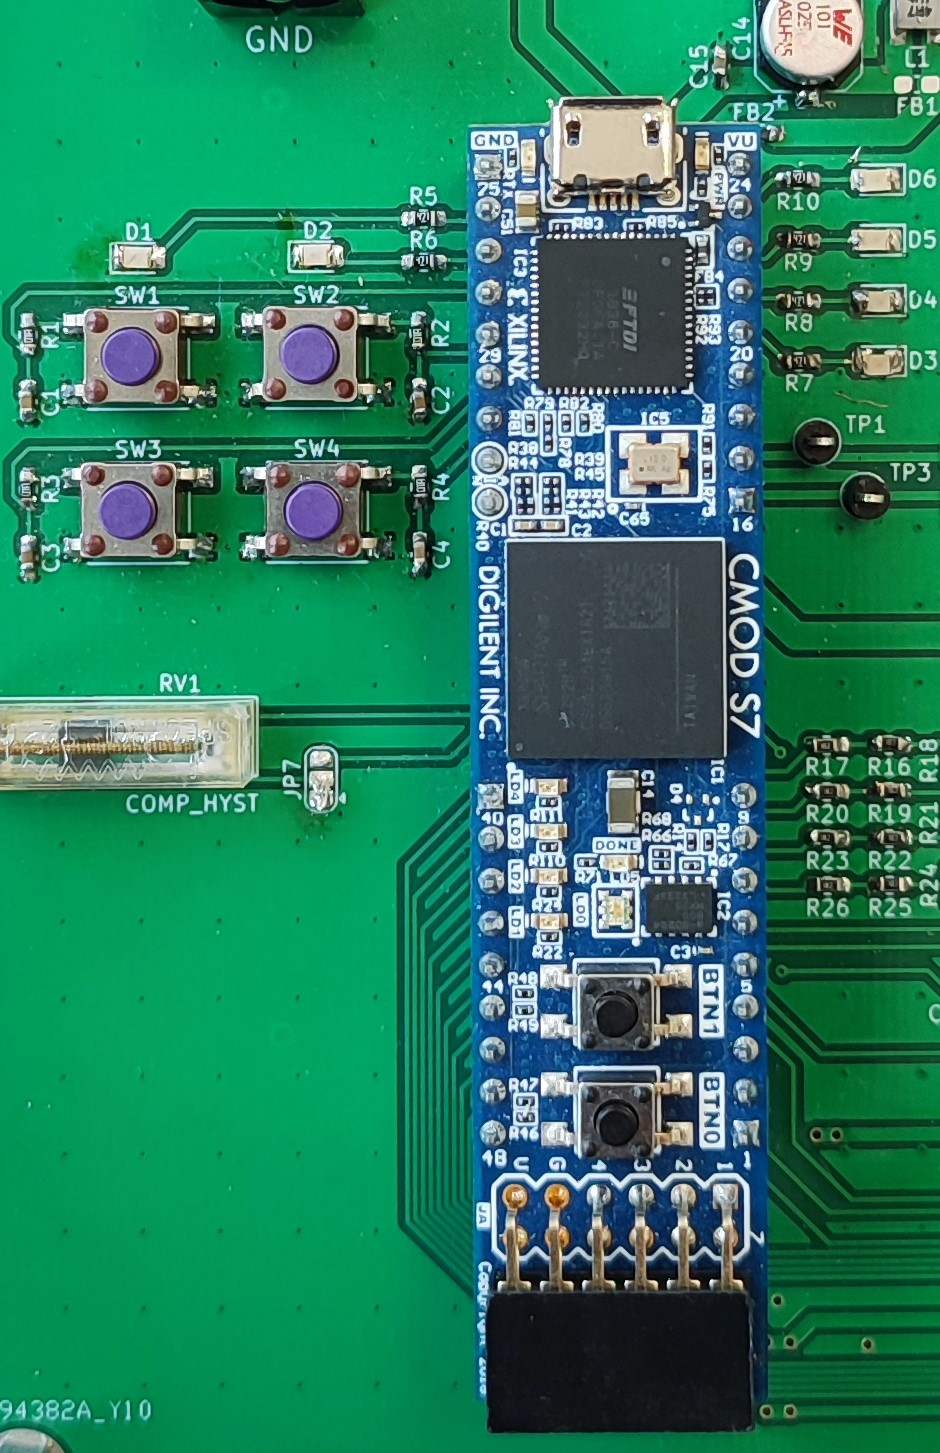
\includegraphics[width=1.0\linewidth]{images/tastenbelegung.jpg}}
	\annotatedFigureBox{0.0873,0.725}{0.1896,0.7877}{B1}{0.0873,0.725}%bl
	\annotatedFigureBox{0.085,0.6163}{0.1886,0.682}{B3}{0.085,0.6163}%bl
	\annotatedFigureBox{0.2782,0.7242}{0.38,0.7905}{B2}{0.2782,0.7242}%bl
	\annotatedFigureBox{0.2836,0.6147}{0.3833,0.686}{B4}{0.2836,0.6147}%bl
	\annotatedFigureBox{0.1167,0.8138}{0.1778,0.832}{D1}{0.1167,0.832}%tl
	\annotatedFigureBox{0.3052,0.8132}{0.3667,0.8364}{D2}{0.3052,0.8364}%tl
	\annotatedFigureBox{0.9081,0.7408}{0.9609,0.7631}{D3}{0.9081,0.7631}%tl
	\annotatedFigureBox{0.9095,0.7828}{0.9625,0.8052}{D4}{0.9095,0.8052}%tl
	\annotatedFigureBox{0.9081,0.8272}{0.9579,0.844}{D5}{0.9081,0.844}%tl
	\annotatedFigureBox{0.905,0.8672}{0.9588,0.8872}{D6}{0.905,0.8872}%tl
	\annotatedFigureBox{0.6144,0.2032}{0.6938,0.3288}{BX}{0.6144,0.2032}%bl
	\annotatedFigureBox{0.568,0.3576}{0.6028,0.4668}{DX}{0.568,0.3576}%bl
	\annotatedFigureBox{0.568,0.3576}{0.6739,0.3856}{DX}{0.568,0.3576}%bl
\end{annotatedFigure}
\caption{Overview of I/O}
\end{minipage}\hfill
\begin{minipage}{0.6\textwidth}
\begin{itemize}
    \item B1: Starts a predefined data or test transmission (depending on Verilog flag)
    \item B2: Enables/disables the VGA.
    \item B3: Decreases the gain by 1.
    \item B4: Increases the gain by 1.
    \item BX: Unassigned push buttons.
    \item D1: Indicates a running communication.
    \item D2: Indicates the status of the VGA (on/off).
    \item D3: Bit 0 (LSB) of the VGA gain.
    \item D4: Bit 1 of the VGA gain.
    \item D5: Bit 2 of the VGA gain.
    \item D6: Bit 3 (MSB) of the VGA gain.
    \item DX: Unassigned LEDs.
\end{itemize}
\end{minipage}

\label{img:tastenbelegung}
\end{figure}
%https://ff.cx/latex-overlay-generator/#/v0.0.1


The \gls{PCB} and \gls{FPGA} offer some basic \gls{IO} for human operators, namely push buttons and \glspl{LED}. While not all have been assigned to a function, the buttons and \glspl{LED} enable the transmission of the predefined data and setting up the VGA to output the amplified differential signal over the BNC connectors, as seen in \cref{img:tastenbelegung}. This enables all key functions which are not dependent on a host computer.


\chapter{Conclusion}
This report shows the design and development of a test \gls{PCB} for ultrasonic communication. Its intended use is the support and testing of a custom ASIC which is powered and operated by ultrasonic communication using piezoelectric transducers.

The resulting implementation features data transmission using a simple \gls{OOK} encoding and data reception, sampling and forwarding with the use of an amplifier, a comparator, an \gls{ADC} and a \gls{FPGA} as its logic core. The platform can be operated in its most basic functionality with its push button and \gls{LED} interface and offers high configurability and sampling features when paired with a host computer. The configurability makes it suitable for interfacing with a variety of piezo elements, only limited by a maximum reception frequency of \SI{5}{\mega\hertz} in the case of the \gls{ADC}, for long sampling durations in the region of up to a few dozen milliseconds and different communication mechanisms. The Verilog code for the \gls{FPGA} logic was designed in order to be as modular as possible in terms of host computer communication and to offer a modifiable basis for different transmission and sampling strategies.

Further work may be directed at implementing these strategies and enhancing the platform through higher sampling frequencies for the comparator and \gls{ADC} and by increasing the transmission speeds to the host computer if needed. Suggestions for such changes were stated in the previous chapter.



% Appendix
% -------------------------------------------------------------------

\setcounter{biburllcpenalty}{7000}
\setcounter{biburlucpenalty}{8000}
% References
\printbibliography

% List of figures:
\listoffigures

% List of listings:
\lstlistoflistings

\end{document}
